\chapter{Design} \label{section:design}
The design phase sets out to elaborate on the scenarios for experiments with IoT device. In these experiments, we compare and combine approaches from industry standards and papers presented in the analysis section. Noted observations are taken into consideration in establishing the plan of measurements and in the construction of the sensor unit. Finally, the network infrastructure layout is provided where we propose optimizations in the functions of the components.

\section{Research questions}
This thesis aims to provide answers to four research questions formulated in broader sense. The focus is primarily on making data flow more efficient in an industrial sensor network that monitors rotating machines. The \textbf{research questions} are:
\begin{enumerate}[label=RQ\arabic*., font=\bfseries]
    \itemsep0pt
	\item Which temporal and spectral features can be extracted from vibration signals to provide the most accurate record of machinery faults?
	\item What is the reduction in transmission goodput when chosen signal features are used?
	\item What accuracies of prediction models can be achieved with various feature subsets?
	\item How can machinery faults be continuously identified and predicted based upon collected events?
\end{enumerate}

\noindent In accomplishing the objectives of our research we propose several \textbf{goals}:
\begin{todolist}
    \itemsep0pt
	\item Statistically and visually describe vibration signals from the Machinery fault database (MauFaulDa).
	\item Establish a list of conditions that should be later investigated in the experimental setting.
	\item Prepare dataset to be used in conjunction with statistical learning models, namely by identifying labels and balancing classes.
	\item Find the best subsets of features in temporal and spectral domain with previously analyzed feature extraction and selection methods.
	\item Evaluate the performance of models described in the diagnostics section with a significant focus on the k-nearest neighbor algorithm.
	\item Combine feature selection with online machine learning model.
	\item Acquire measurements of vibrations from machines in the real environment to form a novel dataset of machinery behavior.
	\item Develop hardware and implement its firmware to obtain such measurement in the quality demanded by vibrodiagnostics standards.
\end{todolist}

However, we leave out from our efforts experiments on the data features calculated from wavelets and peaks in the spectral domain. The reason is that we did not find a way to represent extracted features more succinctly as a single number. We also did not discover a strategy for choosing only the relevant frequency bins. The assembled description is retained to lead further research on that topic. \\

The tasks are associated with certain \textbf{risks} impacting their successful completion. The possible risks are assessed and prioritized. The most notable risk encountered is that the machine in the real environment will not be available for vibration measurements. We successfully eliminated the risk by contacting and establishing collaboration with alternative partners. 

The additional risks are that the repeated measurements will not be consistent and fault modes could not be reliably differentiated and labeled in the dataset because each machine is unique in its structure. Related is the risk that not enough data is obtained from various classes and suggestions made by exploring the MaFaulDa dataset not be applicable in practice. All these risks have to be tracked and regularly reevaluated to achieve our goals.


\section{Dataset exploration}
In establishing the validity of methods to be deployed on the sensor node we explore the MaFaulDa dataset. It is the largest known machinery fault collection, so it is possible to create multiple subsets based on requested conditions. 

One representative recording is first selected in each available fault category. The sample is visualized and statistically described in both temporal and spectral domains. A whole step-by-step procedure is outlined in the activity diagram (Fig.~\ref{fig:design:mafaulda-preprocessing}).

\begin{figure}[ht]
	\centering
	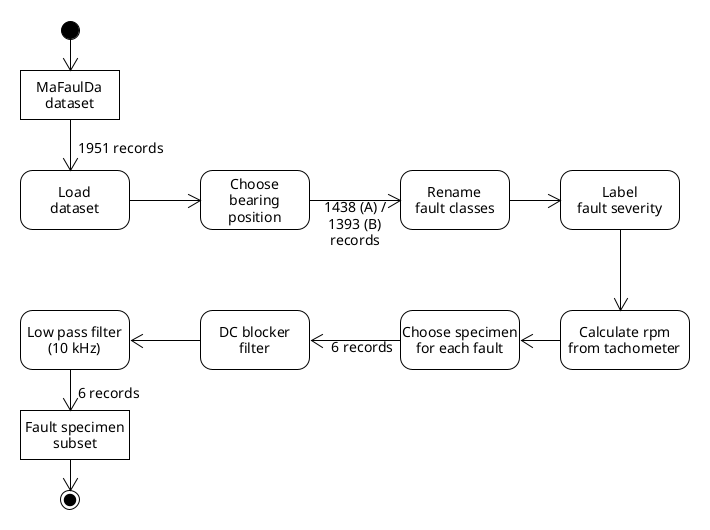
\includegraphics[width=\textwidth]{assets/design/activity-data-exploration.png}
	\caption{Activity diagram of MaFaulDa dataset preprocessing}
	\label{fig:design:mafaulda-preprocessing}
\end{figure}

MaFaulda contains 1951 records labeled with inducted faults of increasing severity. The defects were set up on the machine simulator as is mentioned in the part about datasets. Time series of the triaxial piezoelectric accelerometers in separate files have a sampling frequency of 50 kHz. 

These vibration sensors are placed in two positions. The first placement is around the inner underhang bearing named \emph{A} which is closer to the motor. The second location is around the outer overhang bearing denoted as \emph{B} position.

\subsection{Fault annotations}
The MaFaulDa has annotations altogether for 10 classes of faults of which there is 1 class for fault-free baseline operation, 3 classes for shaft defects, 3 classes for inner bearing defects, and 3 for outer bearing defects. Some categories are redundant or irrelevant for a given sensor position. 

Therefore rotor shaft misalignements in vertical and horizontal directions are merged into one joint group. Depending on the chosen bearing position only records having relevant labels are considered. 

This means that fault classification solely concerns bearing in the direct contact and shaft mechanically passing through it. The bearings affect each other, but the effect on the opposite side should appear via a common interconnection shaft. 

In the end, that leaves \textbf{6 types of labels}: baseline, two shaft faults are imbalance and misalignment, and three bearing faults are cage fault, ball fault, and outer race fault. In the step of choosing the accelerometer location records pointing to the other bearing as a source of the malfunction are discarded. Then the next action renames the labels to be better recognizable and unite the same phenomena.

Groups of identified machine defects are additionally characterized by altered masses attached or motor shaft displacement shifts. The set amount is sorted in ascending order separating \textbf{multiple event severities}. However, the count of severity levels is not identical in every group. Levels are hence scaled into the range between zero and one using a min-max scaler. Scaling is applied to classes separately.

The strength of the recorded response by the underlying defect is also dependent on the shaft \textbf{rotational speed}. Speed in rpm is calculated from pulsed speedometer output. It is the average distance between two successive rising edges: 
\begin{ceqn}\begin{align}
\mathrm{rpm} = 60 \;/\; \overline{\Delta t}
\end{align}\end{ceqn}

\textbf{One specimen waveform} is picked from each fault class to illustrate their superficial differences. Recordings are filtered to get the highest severity levels and around a mean rotation speed of 2500 rpm (42 Hz)  to see the patterns most pronounced. The baseline class sample is chosen according to fixed rotor speed.


\subsection{Signal filters}
The DC component in the three-dimensional vibration signal is removed by subtracting the global mean. Immediately follows a digital IIR Butterworth \textbf{low pass filter} of \nth{5} order with cutoff frequency 10 kHz at -3 dB. 

Before the low pass filter usage, the peak at 20 kHz with sideband was present as an unwanted artifact. It could not have been reliably recorded due to the linear frequency response of the sensor up to 10 kHz. At the same time, such frequency is outside the range of any feasible MEMS accelerometer.

\begin{figure}[ht]
    \centering
    \begin{subfigure}[b]{0.44\textwidth}
        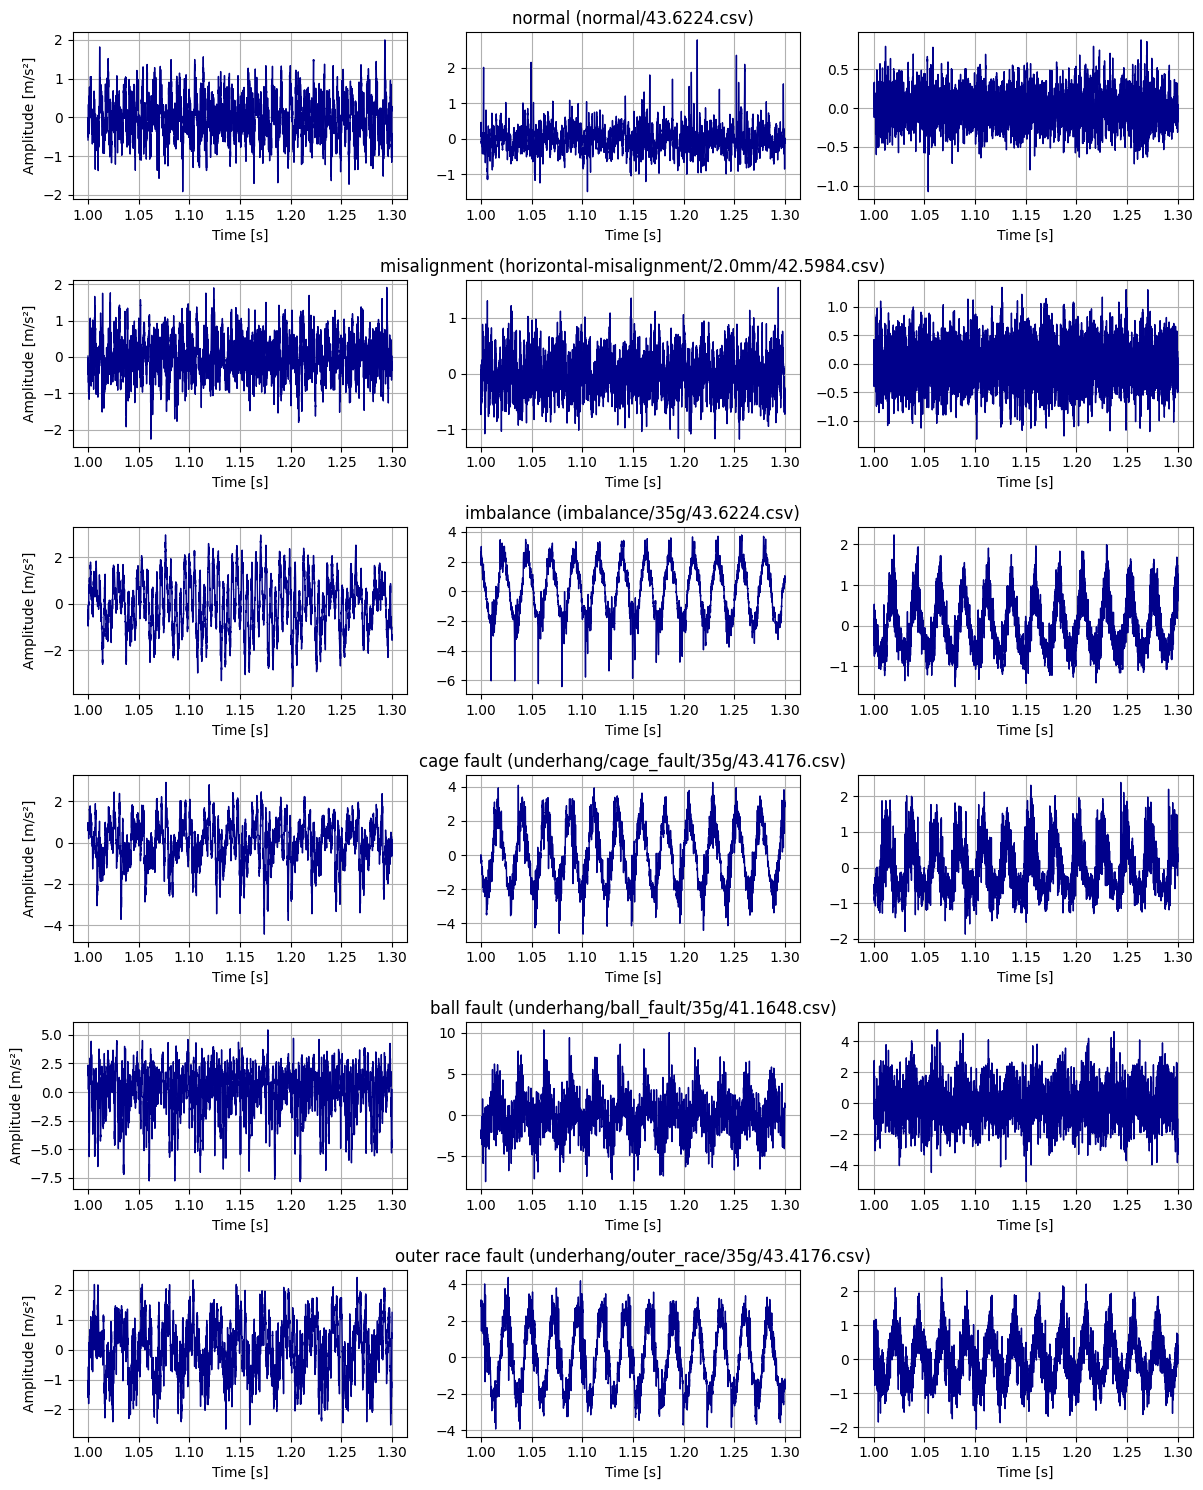
\includegraphics[width=\textwidth]{assets/design/Mafaulda-A-time-waveform.png}
        \caption{Temporal domain waveforms}
        \label{fig:design:fault-temporal-waveform}
    \end{subfigure}
    \hfill
    \begin{subfigure}[b]{0.55\textwidth}
        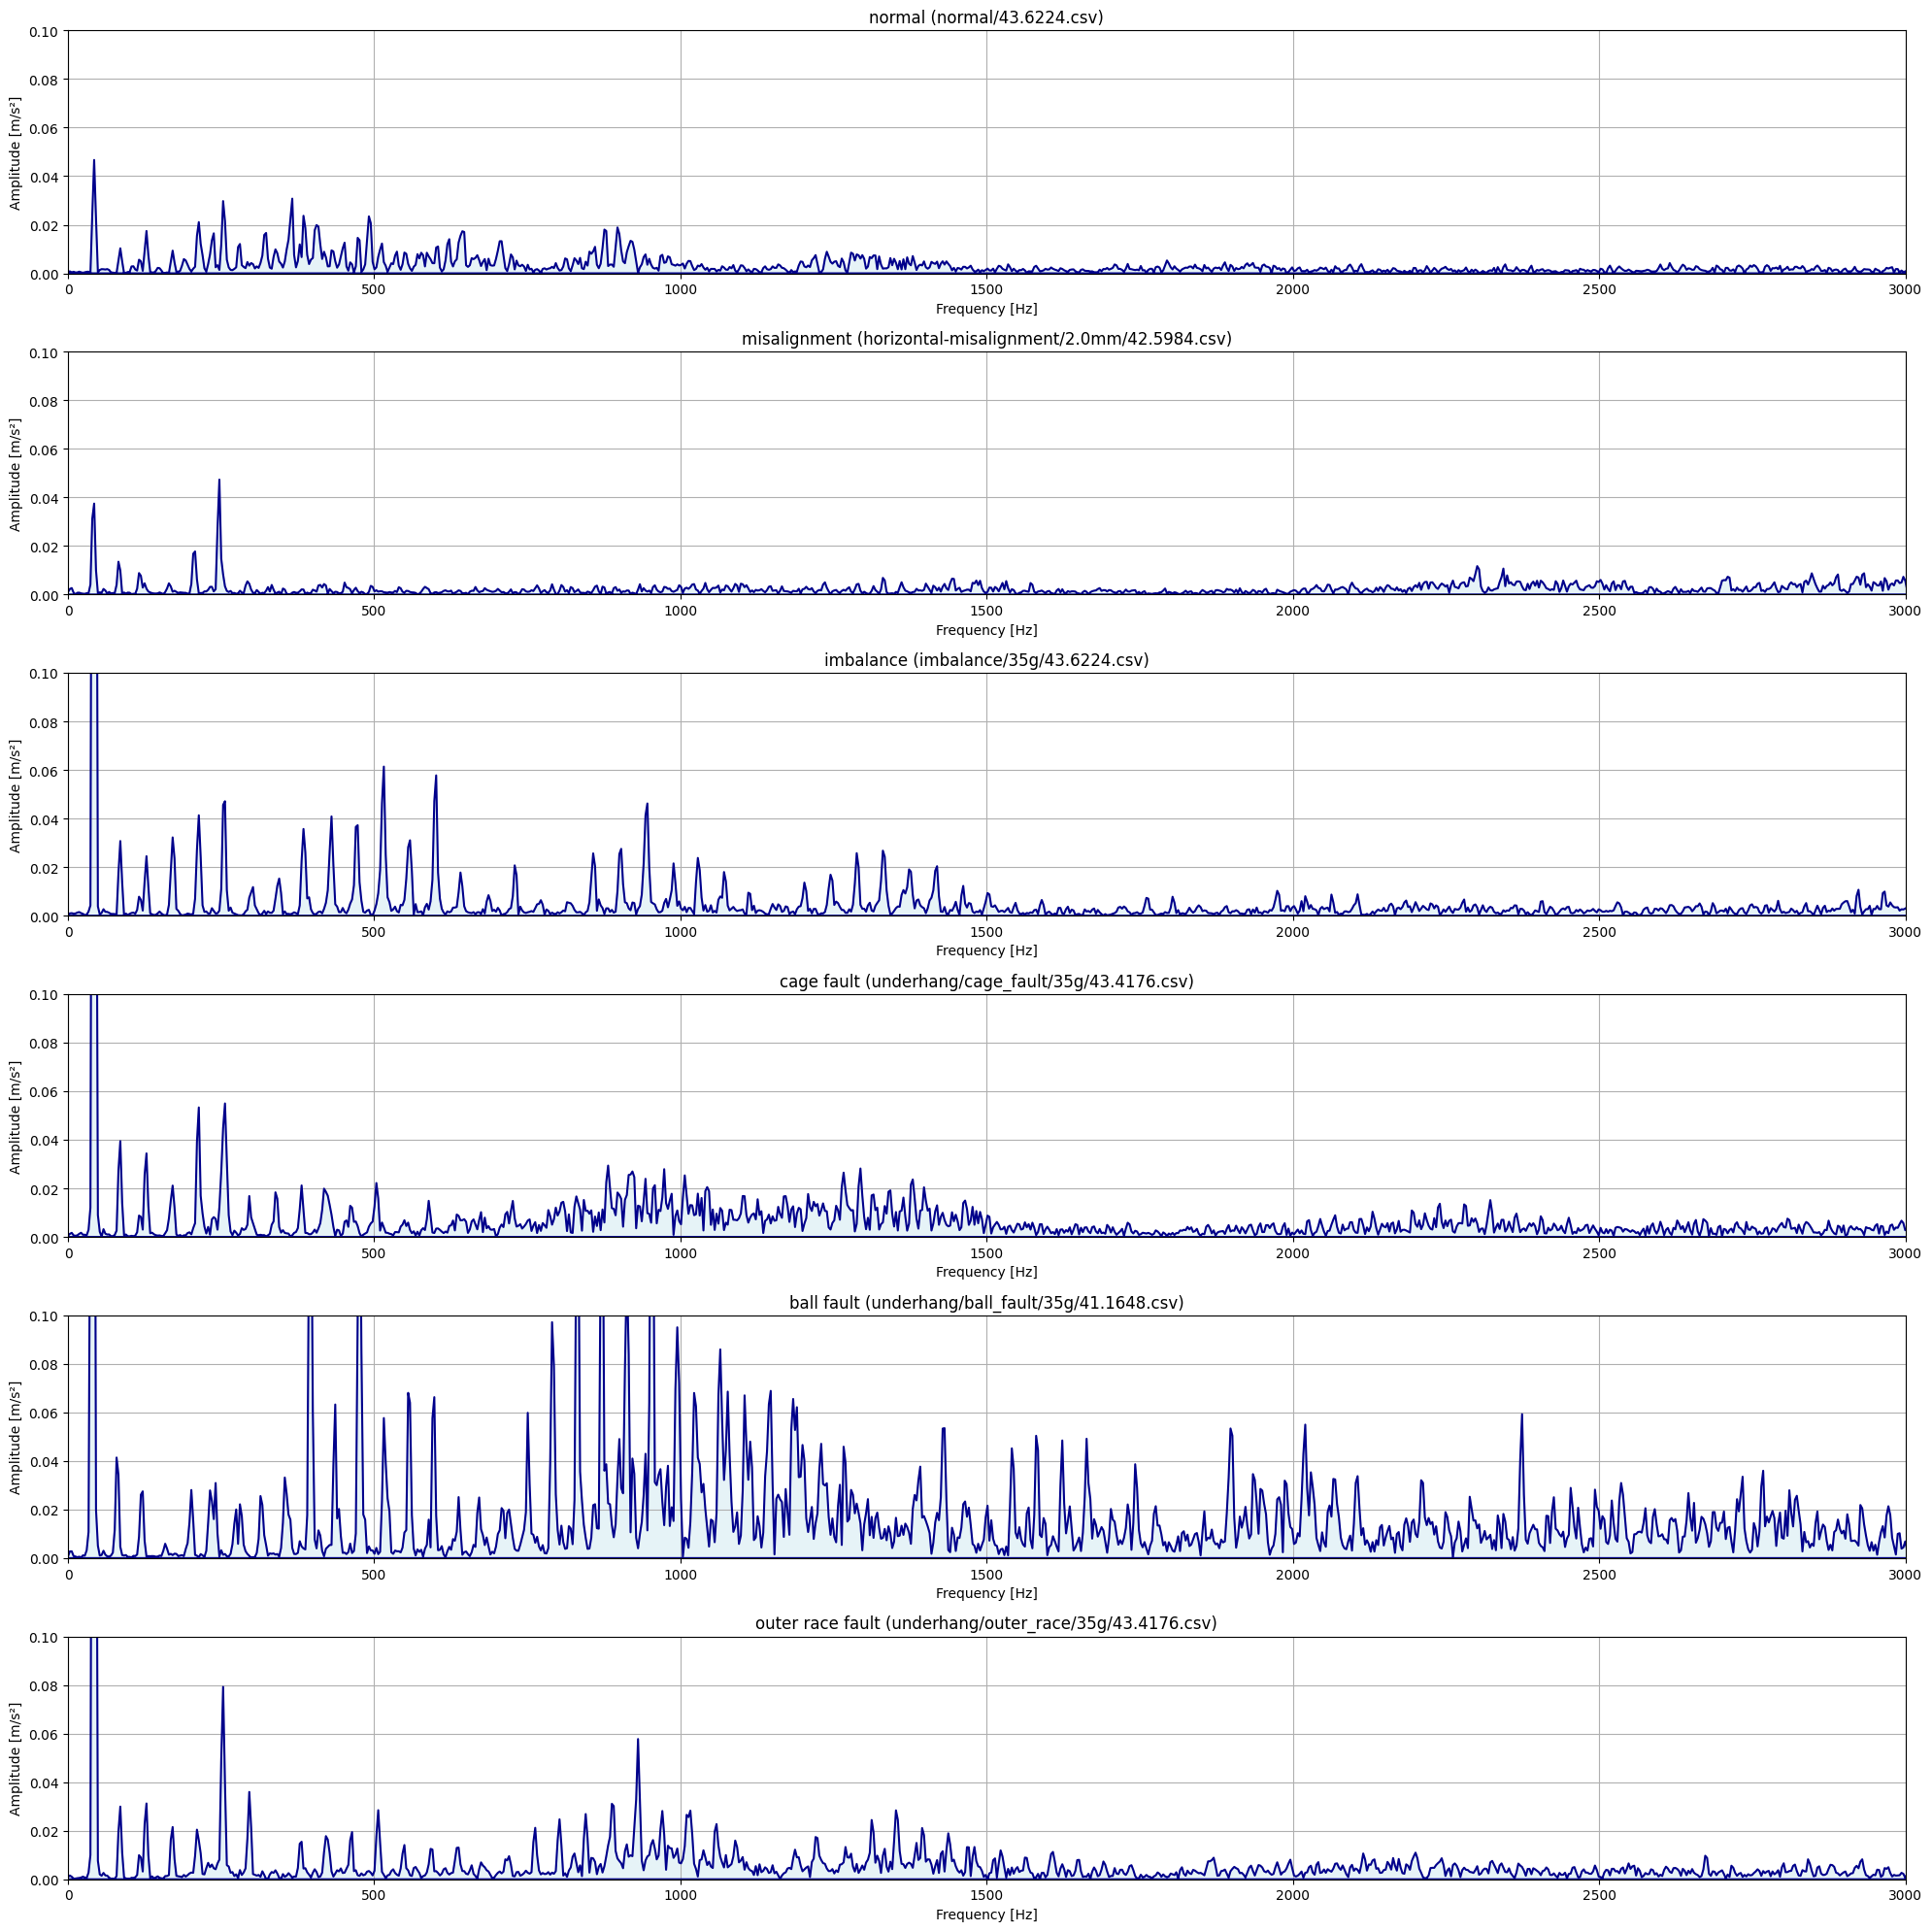
\includegraphics[width=\textwidth]{assets/design/Mafaulda-A-spectrum-Y-axis.png}
        \caption{Spectra in radial direction}
        \label{fig:design:fault-spectral-waveform}
    \end{subfigure} 
    \caption{Inner bearing vibrations (A) for each fault category with the highest fault severity at 2500 rpm}
\end{figure}

Temporal domain waveforms of the 300 ms signal slice are shown in the graphs in Figure \ref{fig:design:fault-temporal-waveform}. Subplots for radial, tangential, and axial directions are laid out in columns from left to right. Amplitudes vary with limits from $\pm 3\; \mathrm{m/s}^2$ in baseline and misalignment time series up to $\pm 11\;\mathrm{m/s}^2$ in case of severe bearing faults. 

The frequency spectrum in Figure \ref{fig:design:fault-spectral-waveform} is obtained by FFT and Hann window of length $2^{14}$. The signal chunk represents an uncertainty box with a duration of approximately 328 ms and a spectral resolution of little over 3 Hz. The graph has been cropped in both axes to make the most important peaks visible.


\subsection{Statistical tests}
The statistical tests and visual checks are conducted to assess \textbf{normality and stationary} of time series. Half a second of amplitude samples are used from every sensor channel. These 25 thousand observations are downsampled tenfold to $2500$ points. 

\textbf{Shapiro-Wilk's test} rejects the null hypothesis (${p < 0.05}$) that data is drawn from normal distribution under most circumstances. The signal has normal distribution when it resembles pink noise lacking a regular pattern or weak exhibition of fault symptoms. \textbf{Quantile–quantile plots} confirm non-normal distribution because of the striking samples tilt to the diagonal line.

\textbf{Augmented Dickey-Fuller test} rejects the null hypothesis of unit root 
(${p < 0.001}$). The same is confirmed with the \textbf{autocorrelation} function shape. It denotes that the stochastic process is stationary as oscillation is bounded.

\section{Feature relevance}
Attributes described in section \ref{section:feature-extraction} are independently summarized from each sensor position and direction. Then similarity score of features is ascertained in relation to a predicted variable. The subset of the strongest predictors is chosen based on the order of their perceived importance.

\subsection{Feature extraction}
Each file in the MaFaulDa contains 6 accelerometer channels. In the feature extraction process sequence of samples is split into 5 parts or 1-second intervals and is passed through the same DC removal filter and low pass filter as in previous experiments. The rotational speed is determined from speedometer pulses belonging to the given chunk. 

Signal chunks are converted afterward into \textbf{10 temporal and 11 spectral features}. Welch's method for spectrum density estimation averaging over $2^{14}$ long FFT segments after Hann windowing is the source for spectral features. The reference implementation of feature calculation is crafted according to mathematical formulas atop of Python packages \emph{SciPy}\footnote{SciPy: \url{https://scipy.org/}} and \emph{Time Series Feature Extraction Library} (TSFEL)\footnote{TSFEL: \url{https://tsfel.readthedocs.io/}}  

The Euclidian norm of feature in the triaxial vector eliminates reliance on the direction of measurement. Value ranges are depicted in Figure \ref{fig:design:feature-range}. 


\begin{figure}[ht]
    \centering
    \begin{subfigure}[b]{\textwidth}
        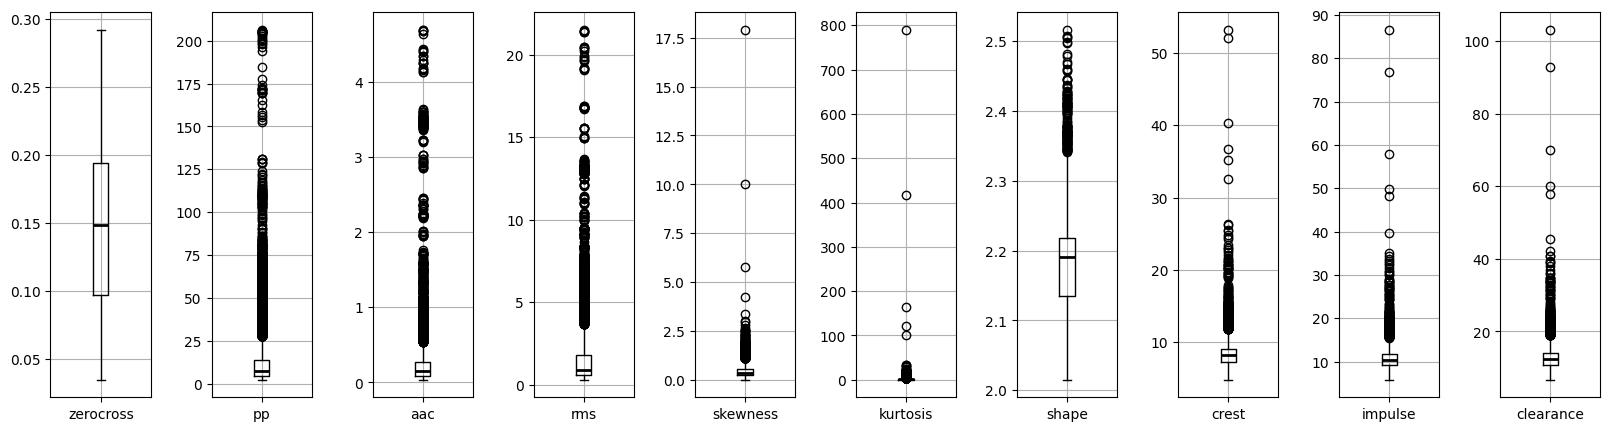
\includegraphics[width=\textwidth]{assets/design/feature-range-temporal.png}
        \caption{Temporal features}
    \end{subfigure}
    \hfill
    \begin{subfigure}[b]{\textwidth}
        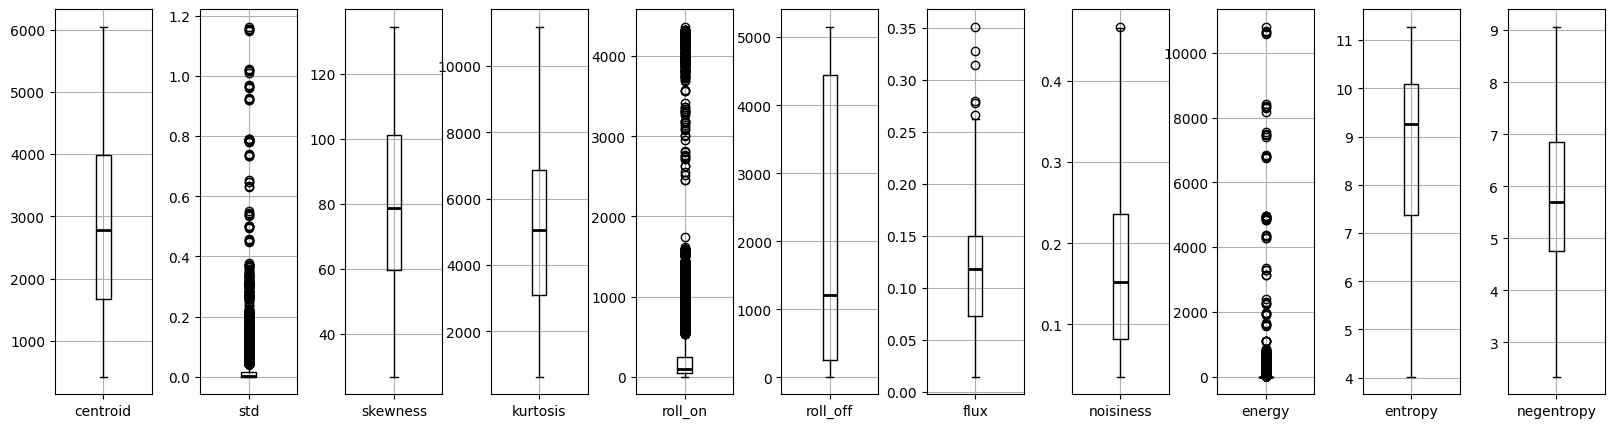
\includegraphics[width=\textwidth]{assets/design/feature-range-spectral.png}
        \caption{Spectral features}
    \end{subfigure}
    \caption{Feature value ranges in inner bearing position (A)}
    \label{fig:design:feature-range}
\end{figure}

Fault labels and their severities come from the directory structure within the dataset. The binary target variable indicating whether to initiate a warning is named to be an anomaly. Anomalies are labeled according to relative fault severity level. We decided to investigate two fault severities having levels above 0.6 and 0.9. The quantity of observation by fault and anomaly severity is shown in Table \ref{tab:observation-counts}. The dataset is substantially unbalanced.

\begin{table}[ht]
\centering
\renewcommand{\arraystretch}{1.2}
\begin{tabular}{rrrrrllll}
\cline{1-3}
\multicolumn{1}{|l|}{\textbf{Fault}}                                                                                          & \multicolumn{1}{l|}{\textbf{Inner bearing (A)}} & \multicolumn{1}{l|}{\textbf{Outer bearing (B)}} \\ \cline{1-3}
\multicolumn{1}{|r|}{\textbf{normal}}                 & \multicolumn{1}{r|}{49 (3\%)}                   & \multicolumn{1}{r|}{49 (4\%)}                    \\ \cline{1-3}
\multicolumn{1}{|r|}{\textbf{misalignment}}           & \multicolumn{1}{r|}{498 (35\%)}                 & \multicolumn{1}{r|}{498 (36\%)}                  \\ \cline{1-3}
\multicolumn{1}{|r|}{\textbf{imbalance}}              & \multicolumn{1}{r|}{333 (23\%)}                 & \multicolumn{1}{r|}{333 (24\%)}                  \\ \cline{1-3}
\multicolumn{1}{|r|}{\textbf{cage fault}}             & \multicolumn{1}{r|}{188 (13\%)}                 & \multicolumn{1}{r|}{188 (13\%)}                  \\ \cline{1-3}
\multicolumn{1}{|r|}{\textbf{ball fault}}             & \multicolumn{1}{r|}{186 (13\%)}                 & \multicolumn{1}{r|}{137 (10\%)}                  \\ \cline{1-3}
\multicolumn{1}{|r|}{\textbf{outer race fault}}       & \multicolumn{1}{r|}{184 (13\%)}                 & \multicolumn{1}{r|}{188 (13\%)}                  \\ \cline{1-3}

\multicolumn{1}{|l|}{\textbf{Anomaly (> 0.6)}}                                                                                          & \multicolumn{1}{l|}{\textbf{Inner bearing (A)}} & \multicolumn{1}{l|}{\textbf{Outer bearing (B)}} \\ \cline{1-3}
\multicolumn{1}{|r|}{\textbf{False}}                                                                            & \multicolumn{1}{r|}{837 (58\%)}                 & \multicolumn{1}{r|}{831 (60\%)}          \\ \cline{1-3}
\multicolumn{1}{|r|}{\textbf{True}}                                                                             & \multicolumn{1}{r|}{601 (42\%)}                 & \multicolumn{1}{r|}{562 (40\%)}          \\ \cline{1-3}

\multicolumn{1}{|l|}{\textbf{Anomaly (> 0.9)}}                                                                                          & \multicolumn{1}{l|}{\textbf{Inner bearing (A)}} & \multicolumn{1}{l|}{\textbf{Outer bearing (B)}} \\ \cline{1-3}
\multicolumn{1}{|r|}{\textbf{False}}                                                                            & \multicolumn{1}{r|}{1227 (85\%)}                 & \multicolumn{1}{r|}{1197 (86\%)}         \\ \cline{1-3}
\multicolumn{1}{|r|}{\textbf{True}}                                                                             & \multicolumn{1}{r|}{211 (15\%)}                 & \multicolumn{1}{r|}{196 (14\%)}         \\ \cline{1-3}
\multicolumn{1}{|r|}{\textbf{Total}}                                                                            & \multicolumn{1}{r|}{\textbf{1438} (100\%)}                       & \multicolumn{1}{r|}{\textbf{1393} (100\%)}               \\ \cline{1-3}
\end{tabular}
\caption{Label count for whole MaFaulDa dataset with recordings split to 5 chunks}
\label{tab:observation-counts}
\end{table}

Pearson's correlation of features to rpm is very low in the whole dataset. In the temporal domain, the correlation coefficient is within an interval of -0.08 to 0.26. In the spectral domain, the correlation to rpm for all FFT window sizes from $2^8$ up to $2^{14}$ is mostly very low from -0.14 up to 0.26, except for centroid being around 0.35.

The correlation among features can reduce prediction power if a pair is elected where $|\mathrm{corr}| > 0.95$. The feature is not added to the subset when the threshold is exceeded. High correlations are more substantial in the temporal domain that are present in these pairs (ordered from the most correlated): \{std, rms\}, \{pp, max\}, \{crest, margin\}, \{impulse, std\}, \{impulse, rms\}. In the spectral domain set \{skewness, kurtosis\} has a strong correlation.

It is assumed that data points spread in each dimension of the feature space could distinguish groups well. The variables that the best explain after min-max scaling total dataset variance in the temporal domain are shape (29\%), RMS, std, max, and pp (each around 15\%). In the spectral domain, variance is the best explained by roll-off (28\%), entropy, skewness, centroid, and kurtosis (each around 12\%).
\begin{figure}[h!]
    \centering
    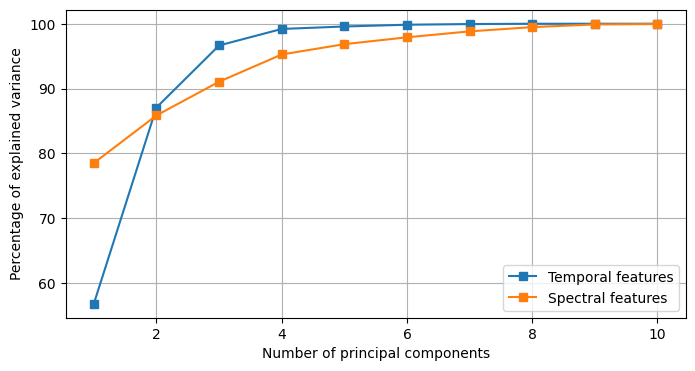
\includegraphics[width=0.8\textwidth]{assets/design/pca-explained-variance.png}
    \caption{Number of principal components to cumulative explained variance percentage in the inner bearing position}
    \label{fig:design:pca-explained-variance} 
\end{figure}

The variables are also more inter-correlated in the temporal domain shown by principal components analysis. For 95\% of the explained variance of PCA 3 components (98.69\%) are needed in the temporal domain whereas 4 in the spectral domain (95.26\%). Figure \ref{fig:design:pca-explained-variance} visualizes cumulative explained variance with an increasing number of principal components.

\begin{figure}[h!]
    \centering
    \begin{subfigure}[b]{0.49\textwidth}
        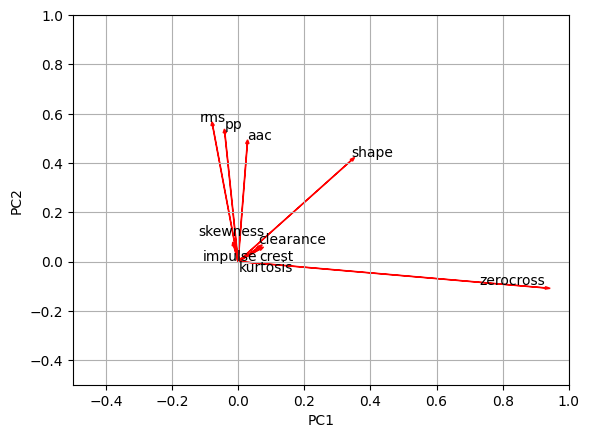
\includegraphics[width=\textwidth]{assets/design/pca-loading-plot-temporal.png}
        \caption{Temporal features}
    \end{subfigure}
    \hfill
    \begin{subfigure}[b]{0.49\textwidth}
        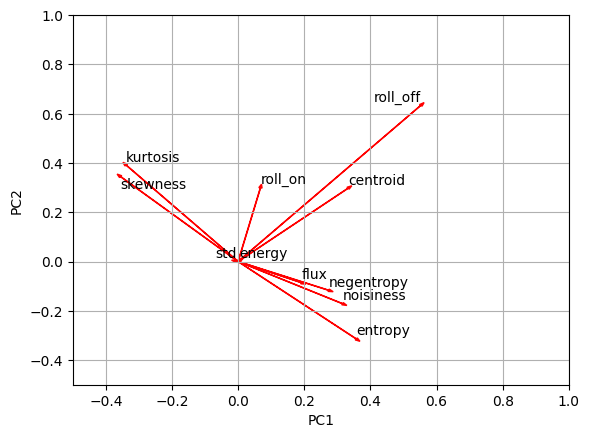
\includegraphics[width=\textwidth]{assets/design/pca-loading-plot-spectral.png}
        \caption{Spectral features}
    \end{subfigure}
    \caption{PCA loading plots for min-max scaled features from the inner bearing position}
    \label{fig:design:pca-loading-plot} 
\end{figure}

PCA loading plots (Fig. \ref{fig:design:pca-loading-plot}) illustrate correlations of features to two principal components. The first PC in the temporal domain focuses on amplitude range (max, rms, pp, std). The second PC mainly describes the impulsiveness of the waveform (shape, impulse, crest, margin). 

However, the distinction between groups is not so apparent for spectral features. Overall chaos in spectra can be attributed to PC1 (flux, entropy, negentropy, noisiness) and the shape of frequency distribution to PC2 (roll-on, roll-off, centroid).


\subsection{Data volume savings}
%TODO
Apparent advantages of feature discovery is data saving. We could do it effetively with PCA but the linear combination is meaningless in reasoning abount which predictors - trend indicators - are decision makers. Data compression must occur on edge device to enable utilize wireless low-power wide area networks (LPWPANs).
Protocol stack may differ therefore we focus on goodput without node configuration metadata and keepalive messages. 

Formula to express compression factor depends on several domain specific parameters:
\begin{itemize}
\itemsep0pt
\item number of machines monitored
\item number of measuremnt places and channels (bearings) - $p_{ch}$ is same in source as output features - devided by dim saved
\item sampling frequency (in Hz) - const. minimum according to faults that warant detection
\item interval between measurements (in s) - $T$
\item duration of valid measurement (in s) - $d$ there can be listening periods which reduc baterry capacity.
\item number of features extracted ($n_{ft}$)
\end{itemize}

Compression ratio ($\mathcal{C}$) for feature space is:
\begin{ceqn}\begin{align}
\mathcal{C} = \frac{n_{ft}}{f_s \cdot d}
\end{align}\end{ceqn}

Compression factor for mafaulda machine simulator
% - (21 * 3) / (3 * 25000 * 1)  (realistic fs because of low pass, we could dowsample by the factor 2) (inverse ratio is data reduction factor =  11904 times less)
% - 3 times less features: (6*3) / (25000*1*3) (83333 times less than original)


 
% Requiremnts classic per bearing (per year): 5s * 20khz * 3dim (365 * 24 = every hour) = (sample is 4/8B just multiplication factor) =  300 kS per measuremnts * 8760 measuremnts = 2.628 GSamples per year per placement
% Frequncy spectra with 1 Hz res = 1*10kHz*3= 30kS = 262.8 MSamples
% All features = 9S  => 78.84 KSamples / year (per year as much as per 3 spectra measurements)

% According to standars is rms velocity enough => indicator of fault (but not of the type)


\subsection{Feature selection}
%TODO
% Methods to find best 3 features
% How many is appropriate?

% COnditions for experminetal setup

%- MaFaulDa features subsets (12 = online, 12 = batch experiments, **Use decision tree ilustation with shorten leaves**
%    - Placement: A, B   - filter only bearing fault for measured bearing, vm and hm to misalign,
%    - Domain: temporal, spectral
%    - Online: no, yes
%    - RPM limit: no, yes (2500 $\pm$ 500)
%    - Classification: fault (multiclass), anomaly (binary - 60%), anomaly( binary - 90%)
%   
%- Validation:
%- **Batch**
%    - Magnitude of 3D feature vector
%    - Balancing dataset with oversampling minority classes
%        - **TODO:Dataset sizes in all experiments (adj/non adjust)**
%    - Hold-out validation - split to train and test set (80/20)
%- **Online**: Order by increaing severity, shuffle samples within severity level
%    - Severity:
%        - Number fault severities by sequence
%        - Keep only decimal numbers in severity
%        - Number severity per group (0 - best, 1 - worst)
%        - Transform severities to range (0, 1)
%     
%- Best features:
%    - Compute metrics: Corr, F stat, MI
%    - Compute Rank product and order descending

% Approval voting

% Ranking


\section{Nearest neighbour classifier}

\subsection{Batch models}


\begin{figure}[ht]
    \centering
    \begin{subfigure}[b]{0.49\textwidth}
        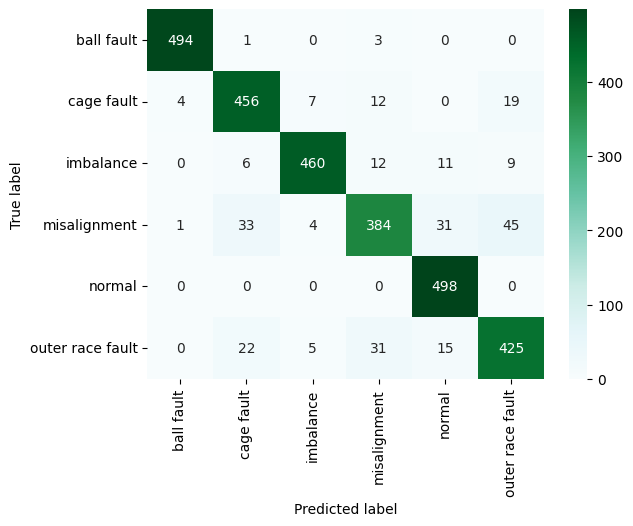
\includegraphics[width=\textwidth]{assets/design/kNN-temporal-confusion-matrix-fault.png}
        \caption{Prediction for 6 fault classes in testing set with temporal domain features}
    \end{subfigure}
    \hfill
    \begin{subfigure}[b]{0.49\textwidth}
        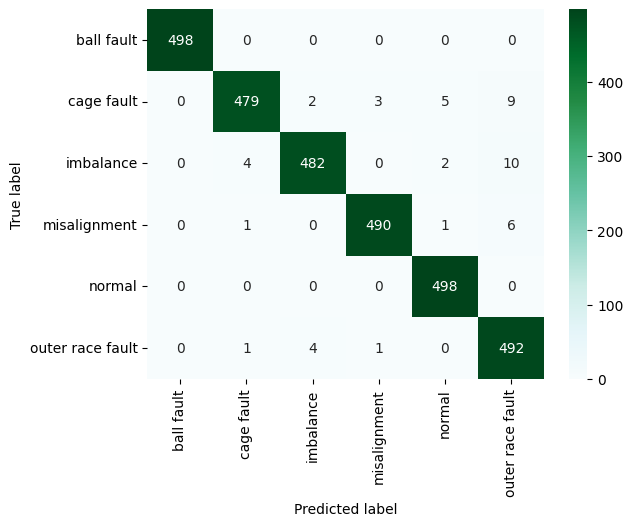
\includegraphics[width=\textwidth]{assets/design/kNN-spectral-confusion-matrix-fault.png}
        \caption{Prediction for 6 fault classes in testing set with spectral domain features}
    \end{subfigure}
    \begin{subfigure}[b]{0.49\textwidth}
        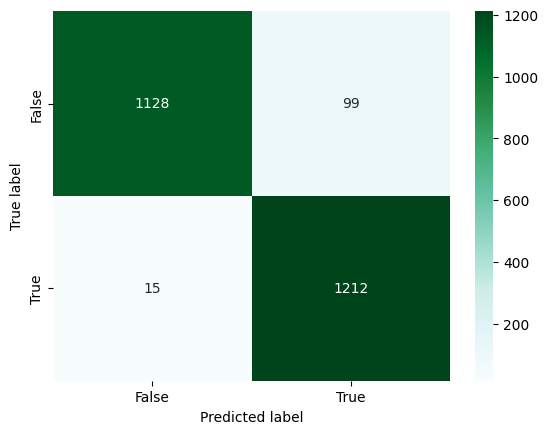
\includegraphics[width=\textwidth]{assets/design/kNN-temporal-confusion-matrix-anomaly90.png}
        \caption{Prediction of high severity anomalies in testing set with temporal domain features}
    \end{subfigure}
    \hfill
    \begin{subfigure}[b]{0.49\textwidth}
        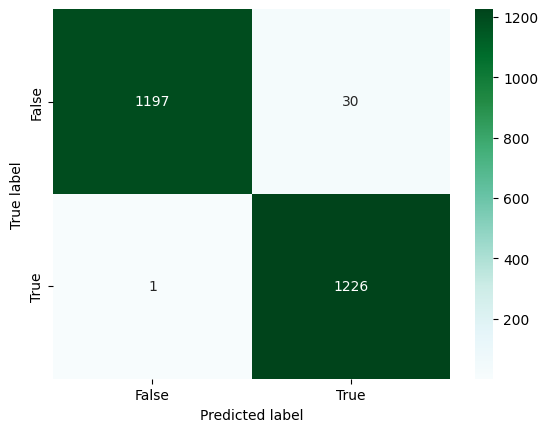
\includegraphics[width=\textwidth]{assets/design/kNN-spectral-confusion-matrix-anomaly90.png}
        \caption{Prediction of high severity anomalies in testing set with spectral domain features}
    \end{subfigure}
    \caption{Confusion matrix of batch kNN algorithm predictions in temporal and spectral domain for two predicted variables measured on inner bearing.}
\end{figure}


\begin{figure}[ht]
    \centering
    \begin{subfigure}[b]{\textwidth}
        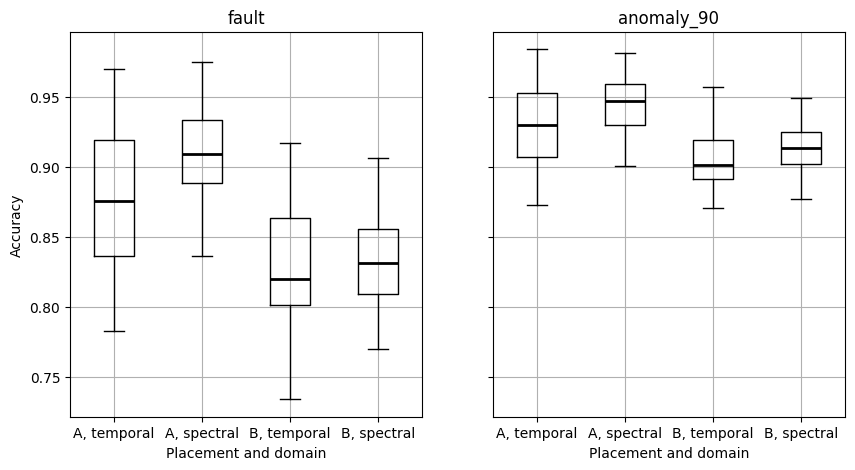
\includegraphics[width=\textwidth]{assets/design/kNN-3-features-combinations-train.png}
        \caption{Testing set}
    \end{subfigure}
    \hfill
    \begin{subfigure}[b]{\textwidth}
        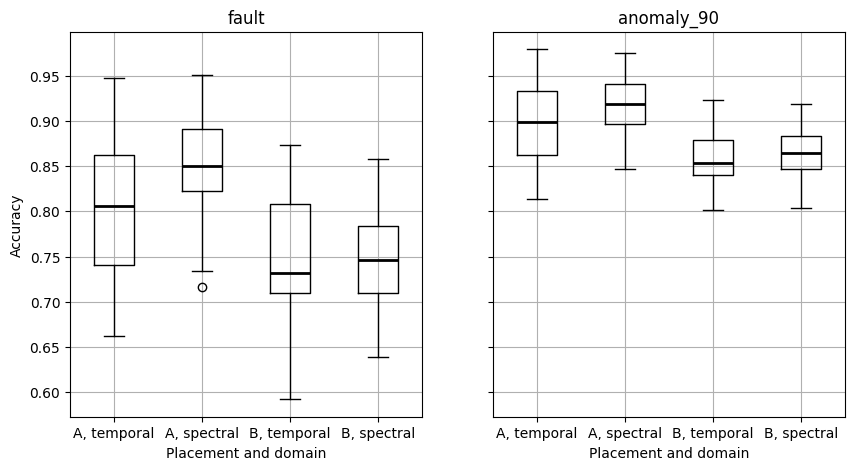
\includegraphics[width=\textwidth]{assets/design/kNN-3-features-combinations-test.png}
        \caption{Training set}
    \end{subfigure}
    \caption{Range of prediction accuracy in all kNN models with subset of 3 features. Subplots show three different predicted variables.}
\end{figure}


\begin{figure}[ht]
    \centering
    \begin{subfigure}[b]{\textwidth}
        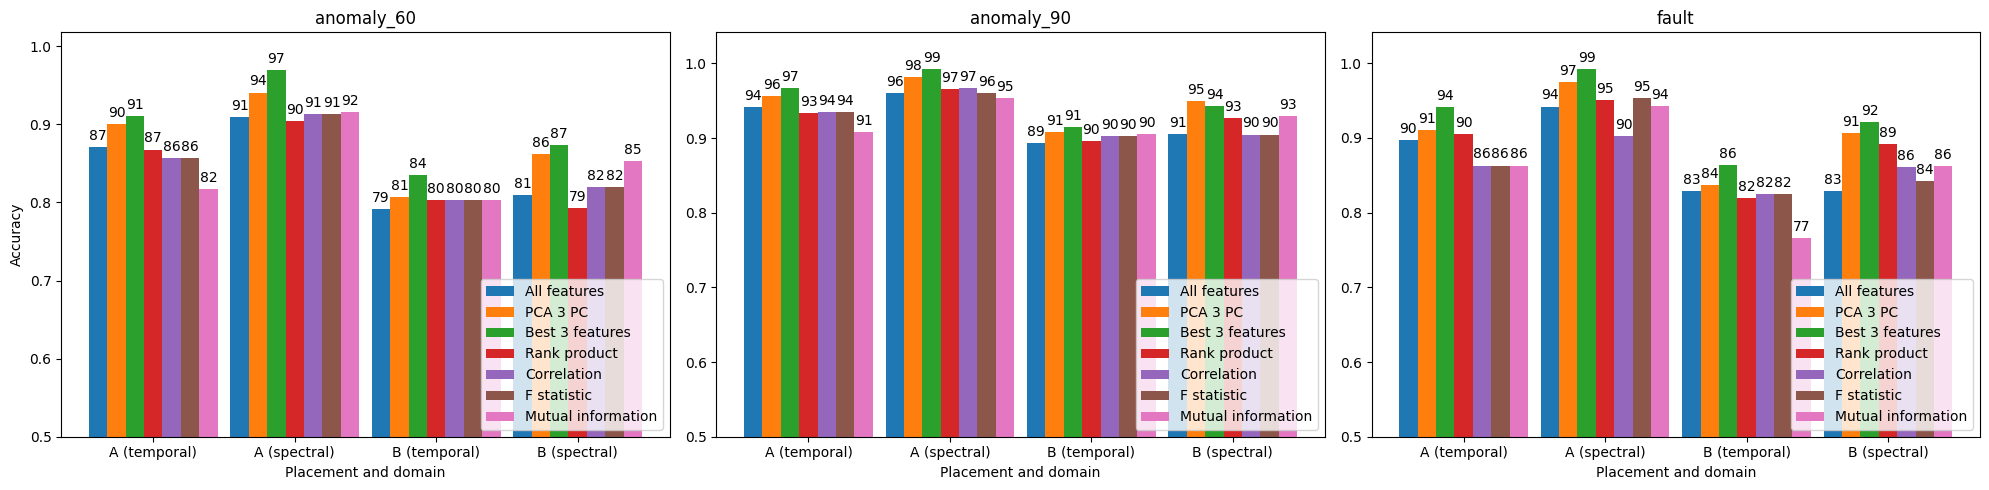
\includegraphics[width=\textwidth]{assets/design/kNN-feature-selection-predictions-train.png}
        \caption{Testing set}
    \end{subfigure}
    \hfill
    \begin{subfigure}[b]{\textwidth}
        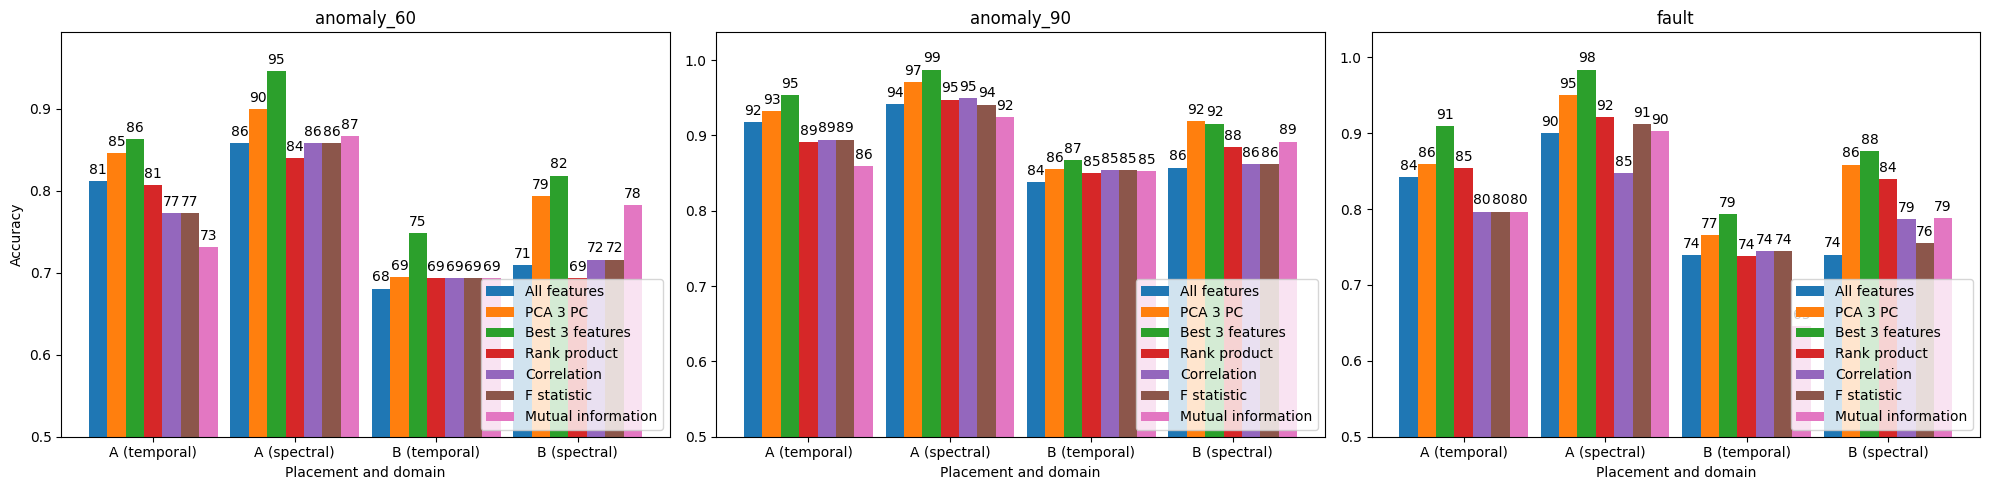
\includegraphics[width=\textwidth]{assets/design/kNN-feature-selection-predictions-test.png}
        \caption{Training set}
    \end{subfigure} 
    \caption{Batch kNN algorithm prediction accuracy with various feature sets.}
\end{figure}

% Number of neighbors (graphs)


\subsection{Online models}

\begin{figure}[ht]
    \centering
    \begin{subfigure}[b]{0.49\textwidth}
        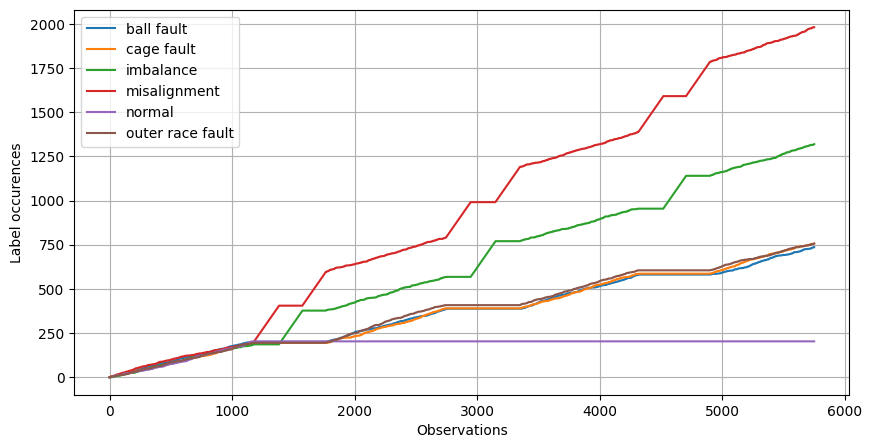
\includegraphics[width=\textwidth]{assets/design/Online-event-ordering-fault-train.png}
        \caption{Training set and fault as predicted variable}
    \end{subfigure}
    \hfill
    \begin{subfigure}[b]{0.49\textwidth}
        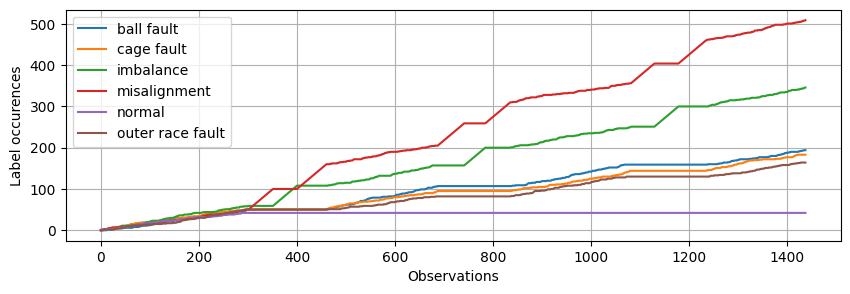
\includegraphics[width=\textwidth]{assets/design/Online-event-ordering-fault-test.png}
        \caption{Testing set and fault as predicted variable}
    \end{subfigure}
    \begin{subfigure}[b]{0.49\textwidth}
        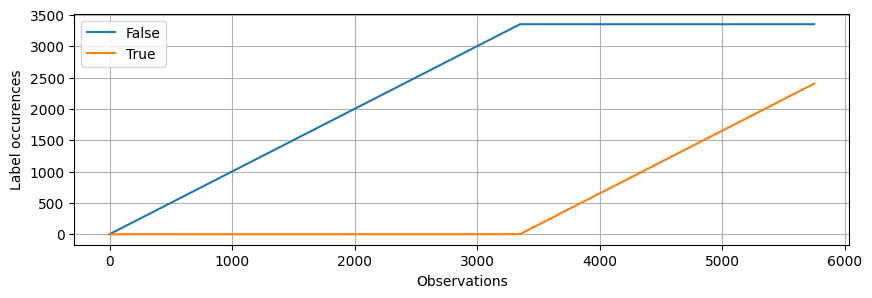
\includegraphics[width=\textwidth]{assets/design/Online-event-ordering-anomaly60-train.png}
        \caption{Training set and medium anomaly severity as predicted variable}
    \end{subfigure}
    \hfill
    \begin{subfigure}[b]{0.49\textwidth}
        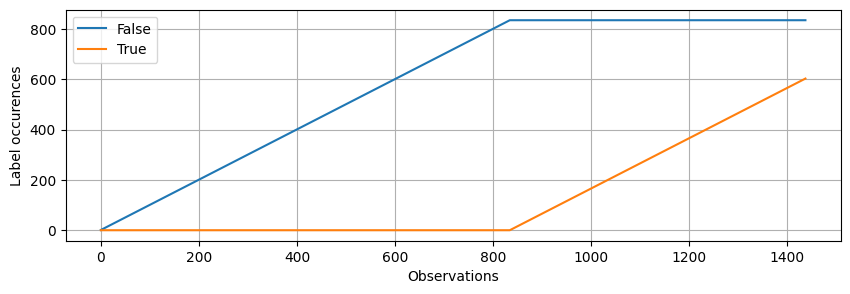
\includegraphics[width=\textwidth]{assets/design/Online-event-ordering-anomaly60-test.png}
        \caption{Training set and medium anomaly severity as predicted variable}
    \end{subfigure}
    \caption{Label order in progressive valuation}
\end{figure}


\begin{figure}[ht]
    \centering
    \begin{subfigure}[b]{0.49\textwidth}
        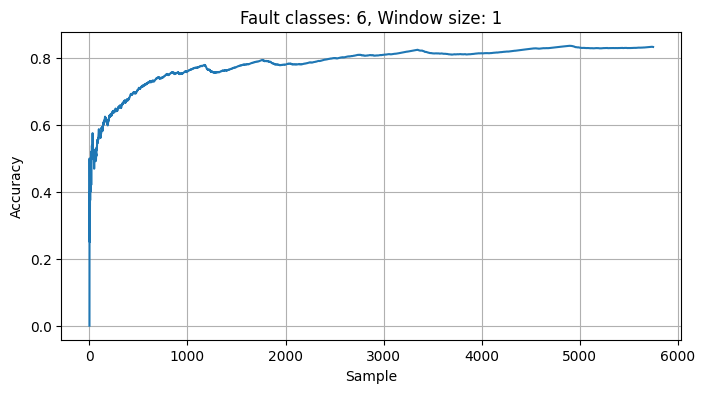
\includegraphics[width=\textwidth]{assets/design/gradual-learning-temporal-domain-fault.png}
        \caption{}
    \end{subfigure}
    \hfill
    \begin{subfigure}[b]{0.49\textwidth}
        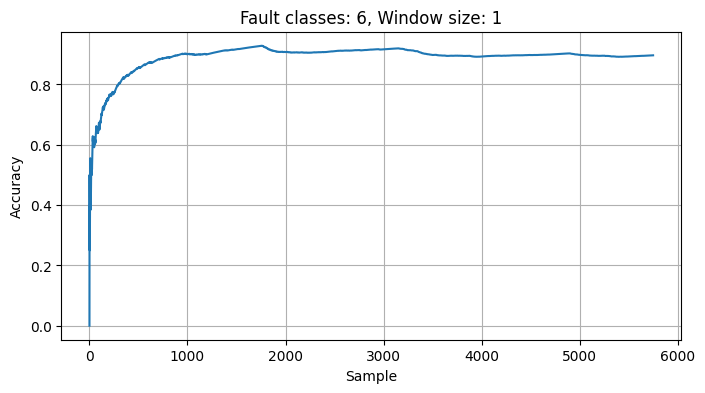
\includegraphics[width=\textwidth]{assets/design/gradual-learning-spectral-domain-fault.png}
        \caption{}
    \end{subfigure}
    \begin{subfigure}[b]{0.49\textwidth}
        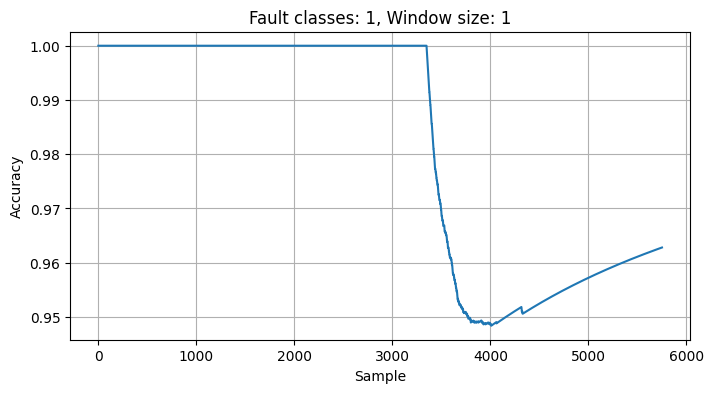
\includegraphics[width=\textwidth]{assets/design/gradual-learning-temporal-domain-anomaly60.png}
        \caption{}
    \end{subfigure}
    \hfill
    \begin{subfigure}[b]{0.49\textwidth}
        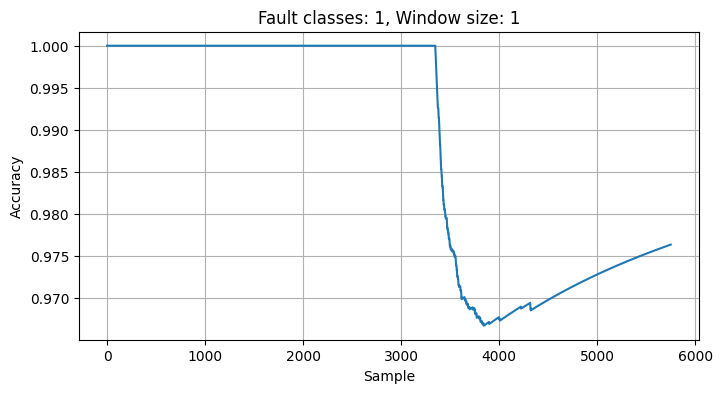
\includegraphics[width=\textwidth]{assets/design/gradual-learning-spectral-domain-anomaly60.png}
        \caption{}
    \end{subfigure}
    \caption{Gradual learning}
\end{figure}


\begin{figure}[ht]
    \centering
    \begin{subfigure}[b]{0.49\textwidth}
        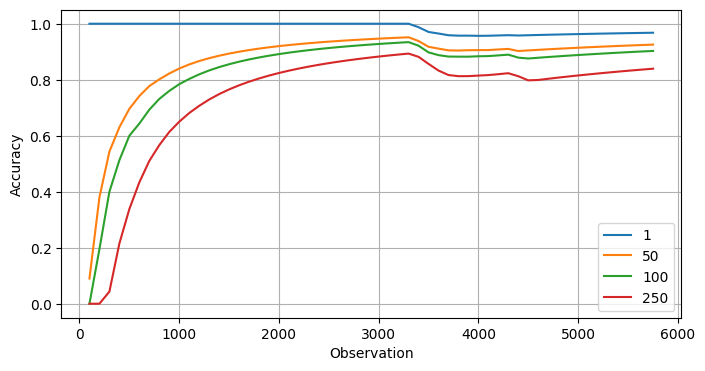
\includegraphics[width=\textwidth]{assets/design/gradual-learning-accuracy-delay-temporal-domain-fault.png}
        \caption{}
    \end{subfigure}
    \hfill
    \begin{subfigure}[b]{0.49\textwidth}
        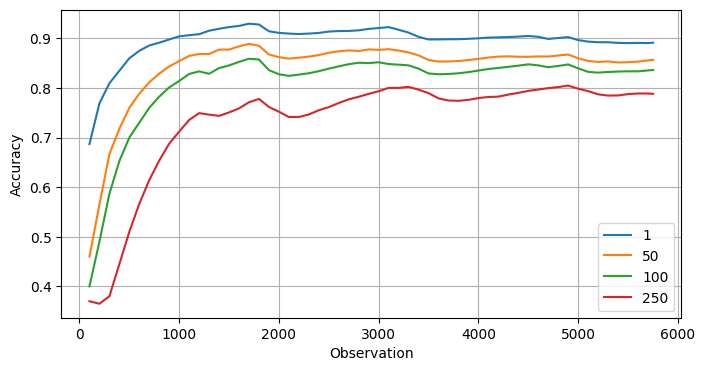
\includegraphics[width=\textwidth]{assets/design/gradual-learning-accuracy-delay-spectral-domain-fault.png}
        \caption{}
    \end{subfigure}
    \begin{subfigure}[b]{0.49\textwidth}
        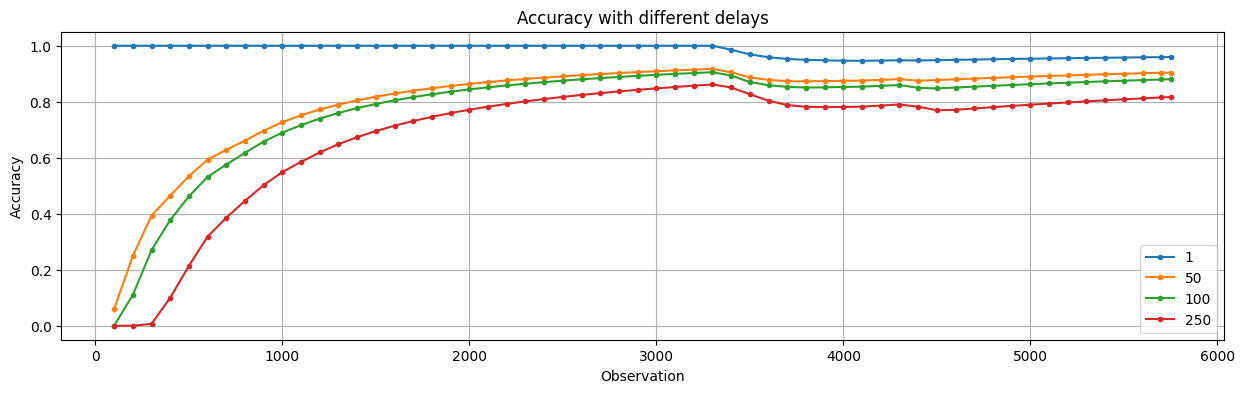
\includegraphics[width=\textwidth]{assets/design/gradual-learning-accuracy-delay-temporal-domain-anomaly60.png}
        \caption{}
    \end{subfigure}
    \hfill
    \begin{subfigure}[b]{0.49\textwidth}
        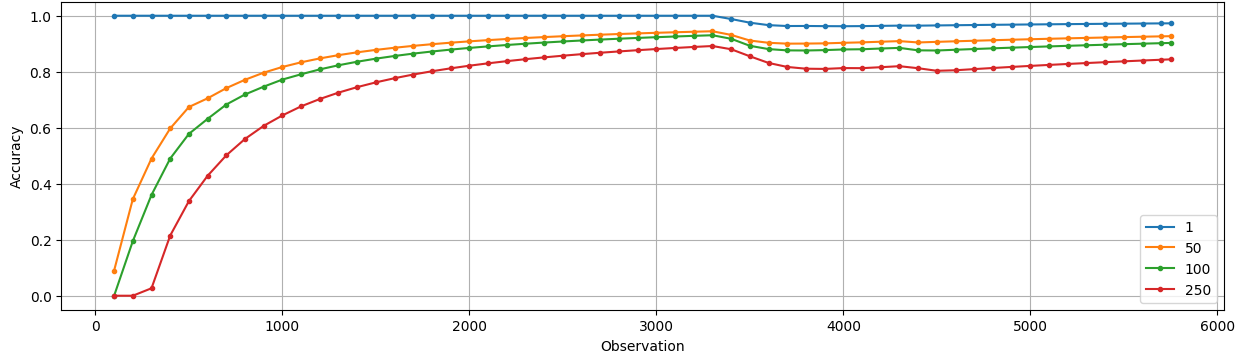
\includegraphics[width=\textwidth]{assets/design/gradual-learning-accuracy-delay-spectral-domain-anomaly60.png}
        \caption{}
    \end{subfigure}
    \caption{Gradual learning accuracy with delay}
\end{figure}



\begin{figure}[ht]
    \centering
    \begin{subfigure}[b]{0.49\textwidth}
        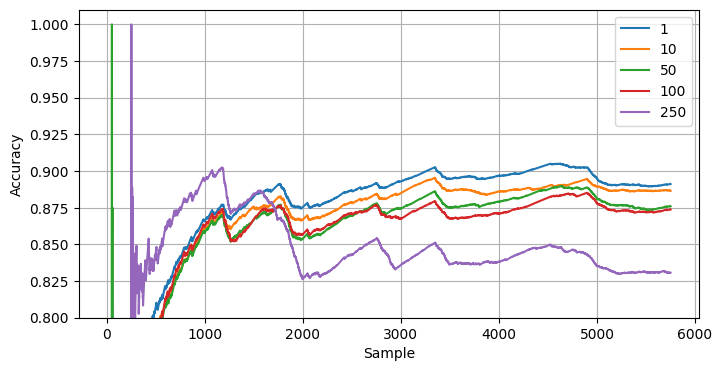
\includegraphics[width=\textwidth]{assets/design/gradual-learning-delay-temporal-domain-fault.png}
        \caption{}
    \end{subfigure}
    \hfill
    \begin{subfigure}[b]{0.49\textwidth}
        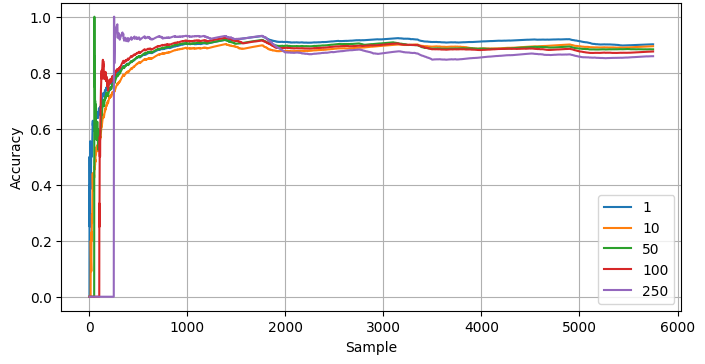
\includegraphics[width=\textwidth]{assets/design/gradual-learning-delay-spectral-domain-fault.png}
        \caption{}
    \end{subfigure}
    \begin{subfigure}[b]{0.49\textwidth}
        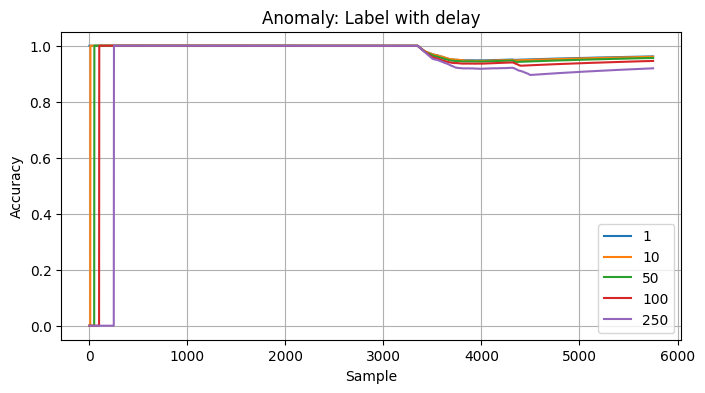
\includegraphics[width=\textwidth]{assets/design/gradual-learning-delay-temporal-domain-anomaly60.png}
        \caption{}
    \end{subfigure}
    \hfill
    \begin{subfigure}[b]{0.49\textwidth}
        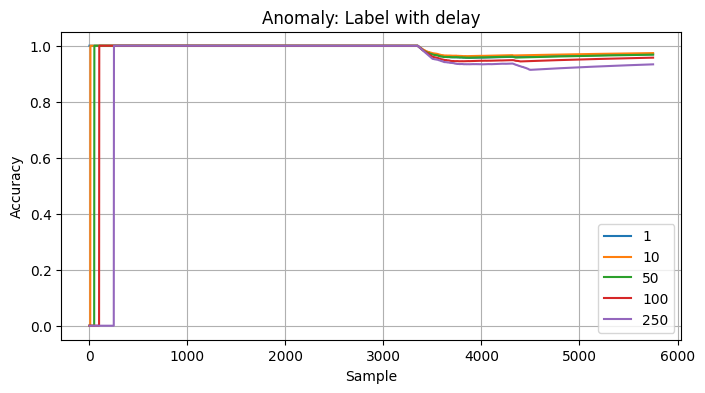
\includegraphics[width=\textwidth]{assets/design/gradual-learning-delay-spectral-domain-anomaly60.png}
        \caption{}
    \end{subfigure}
    \caption{Gradual learning with delay}
\end{figure}



\begin{figure}[ht]
    \centering
    \begin{subfigure}[b]{0.49\textwidth}
        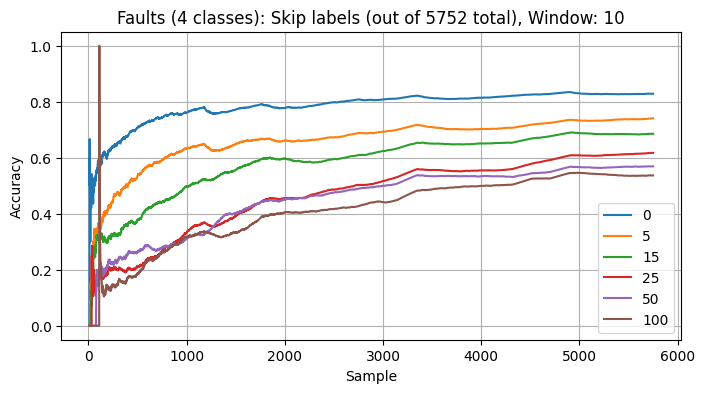
\includegraphics[width=\textwidth]{assets/design/gradual-learning-skip-temporal-domain-fault.png}
        \caption{}
    \end{subfigure}
    \hfill
    \begin{subfigure}[b]{0.49\textwidth}
        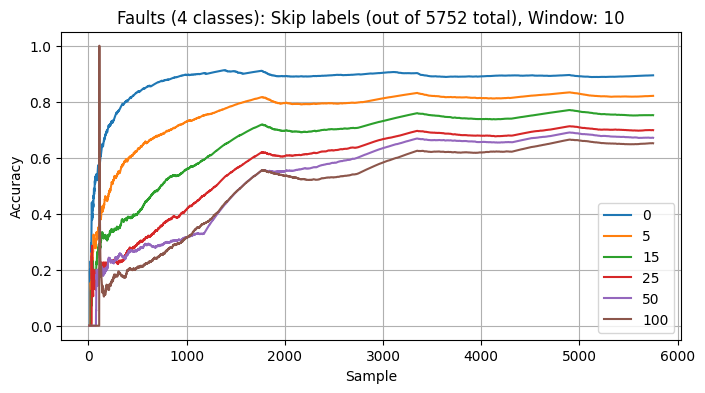
\includegraphics[width=\textwidth]{assets/design/gradual-learning-skip-spectral-domain-fault.png}
        \caption{}
    \end{subfigure}
    \begin{subfigure}[b]{0.49\textwidth}
        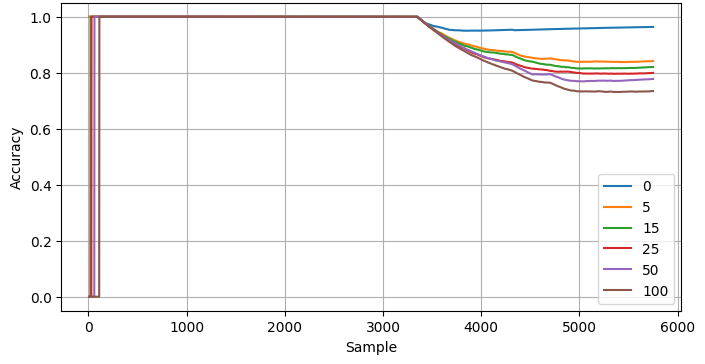
\includegraphics[width=\textwidth]{assets/design/gradual-learning-skip-temporal-domain-anomaly60.png}
        \caption{}
    \end{subfigure}
    \hfill
    \begin{subfigure}[b]{0.49\textwidth}
        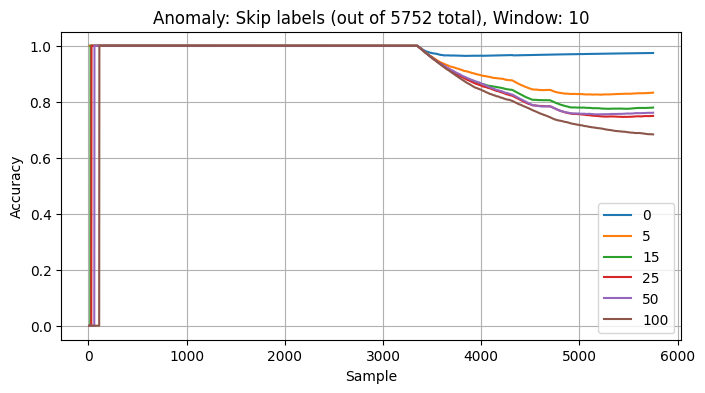
\includegraphics[width=\textwidth]{assets/design/gradual-learning-skip-spectral-domain-anomaly60.png}
        \caption{}
    \end{subfigure}
    \caption{Gradual learning and skip labels}
\end{figure}



\begin{figure}[ht]
    \centering
    \begin{subfigure}[b]{0.49\textwidth}
        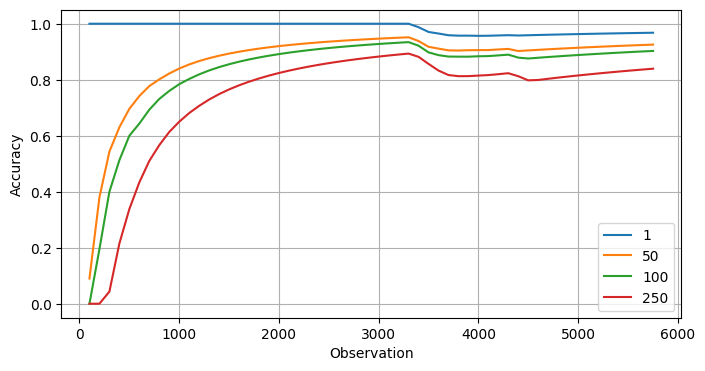
\includegraphics[width=\textwidth]{assets/design/gradual-learning-accuracy-delay-temporal-domain-fault.png}
        \caption{}
    \end{subfigure}
    \hfill
    \begin{subfigure}[b]{0.49\textwidth}
        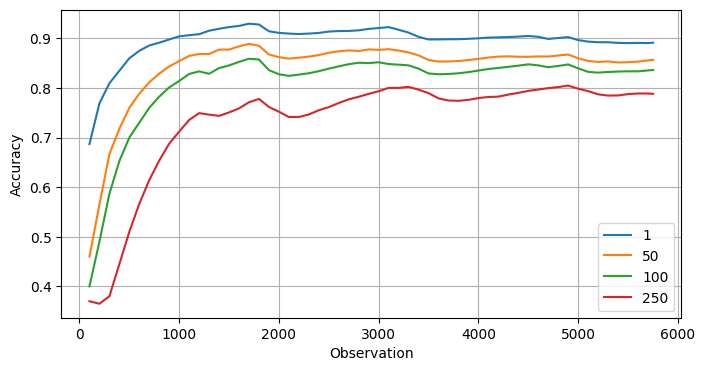
\includegraphics[width=\textwidth]{assets/design/gradual-learning-accuracy-delay-spectral-domain-fault.png}
        \caption{}
    \end{subfigure}
    \begin{subfigure}[b]{0.49\textwidth}
        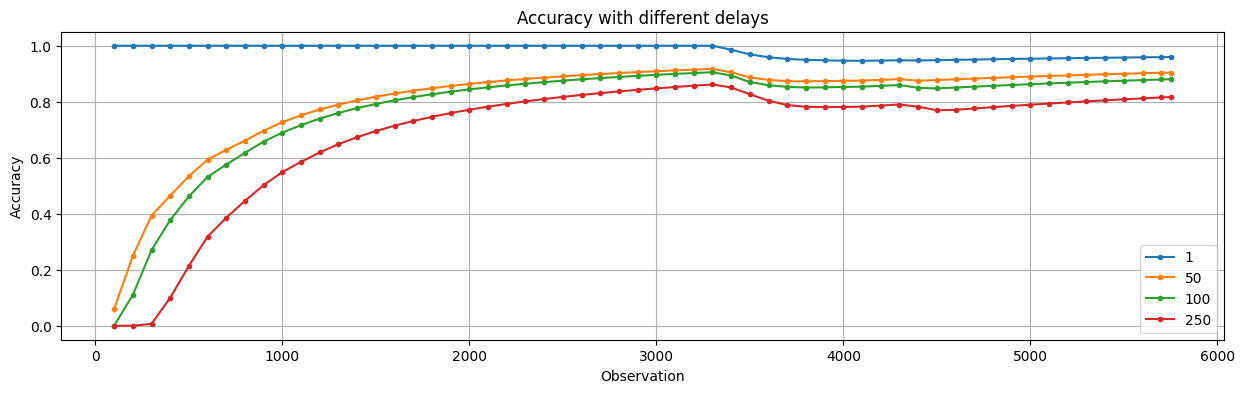
\includegraphics[width=\textwidth]{assets/design/gradual-learning-accuracy-delay-temporal-domain-anomaly60.png}
        \caption{}
    \end{subfigure}
    \hfill
    \begin{subfigure}[b]{0.49\textwidth}
        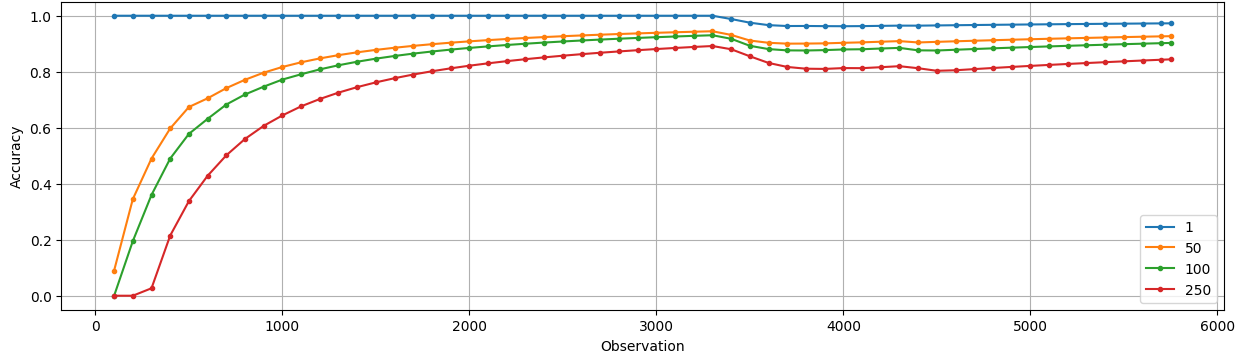
\includegraphics[width=\textwidth]{assets/design/gradual-learning-accuracy-delay-spectral-domain-anomaly60.png}
        \caption{}
    \end{subfigure}
    \caption{Gradual learning accuracy with delay}
\end{figure}



\begin{figure}[ht]
    \centering
    \begin{subfigure}[b]{\textwidth}
        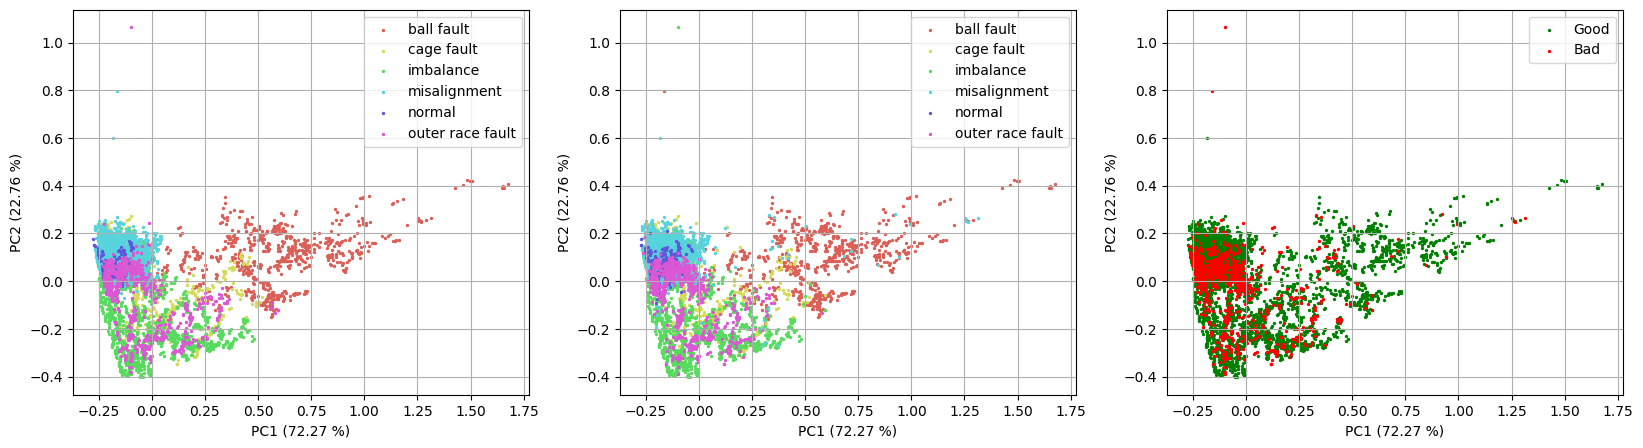
\includegraphics[width=\textwidth]{assets/design/pca-scatter-online-fault-temporal.png}
        \caption{}
    \end{subfigure}
    \hfill
    \begin{subfigure}[b]{\textwidth}
        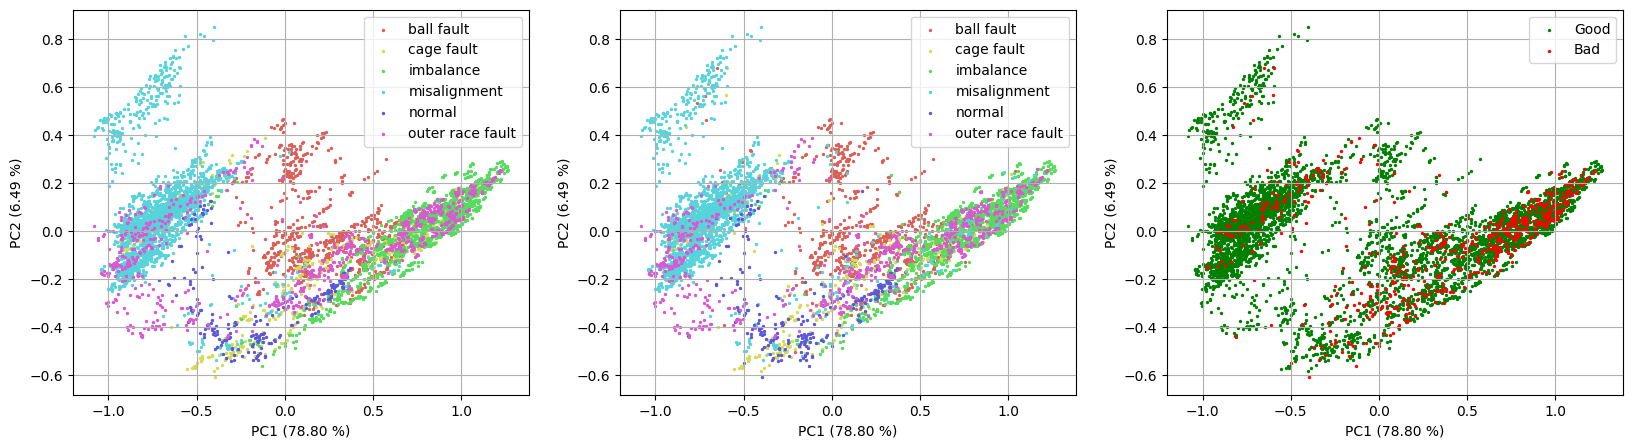
\includegraphics[width=\textwidth]{assets/design/pca-scatter-online-fault-spectral.png}
        \caption{}
    \end{subfigure}
    \begin{subfigure}[b]{\textwidth}
        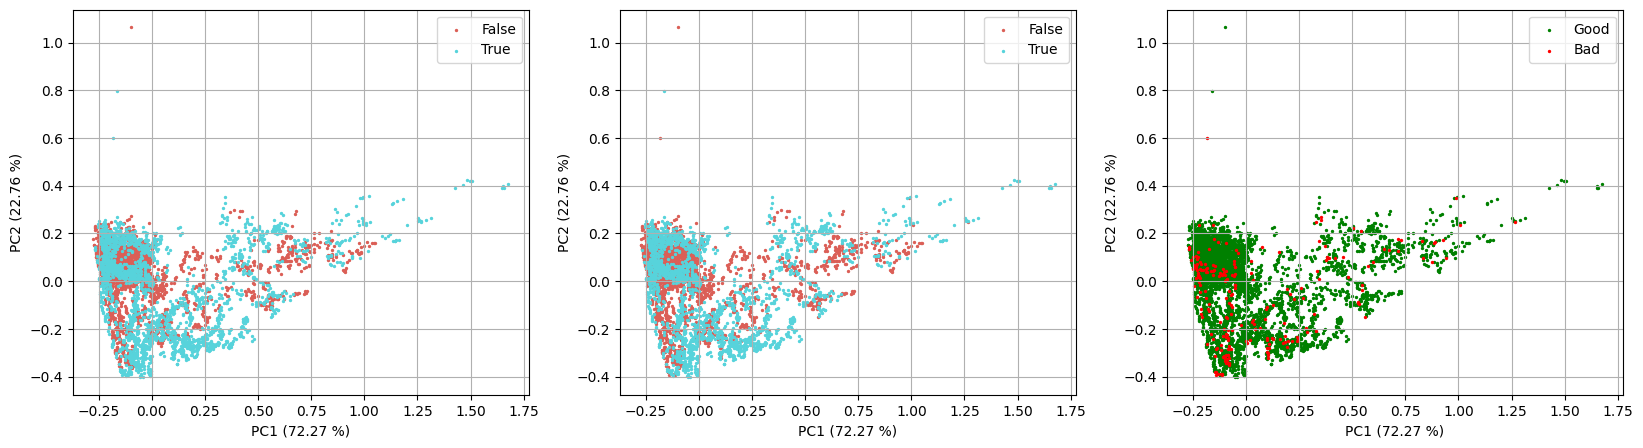
\includegraphics[width=\textwidth]{assets/design/pca-scatter-online-anomaly60-temporal.png}
        \caption{}
    \end{subfigure}
    \hfill
    \begin{subfigure}[b]{\textwidth}
        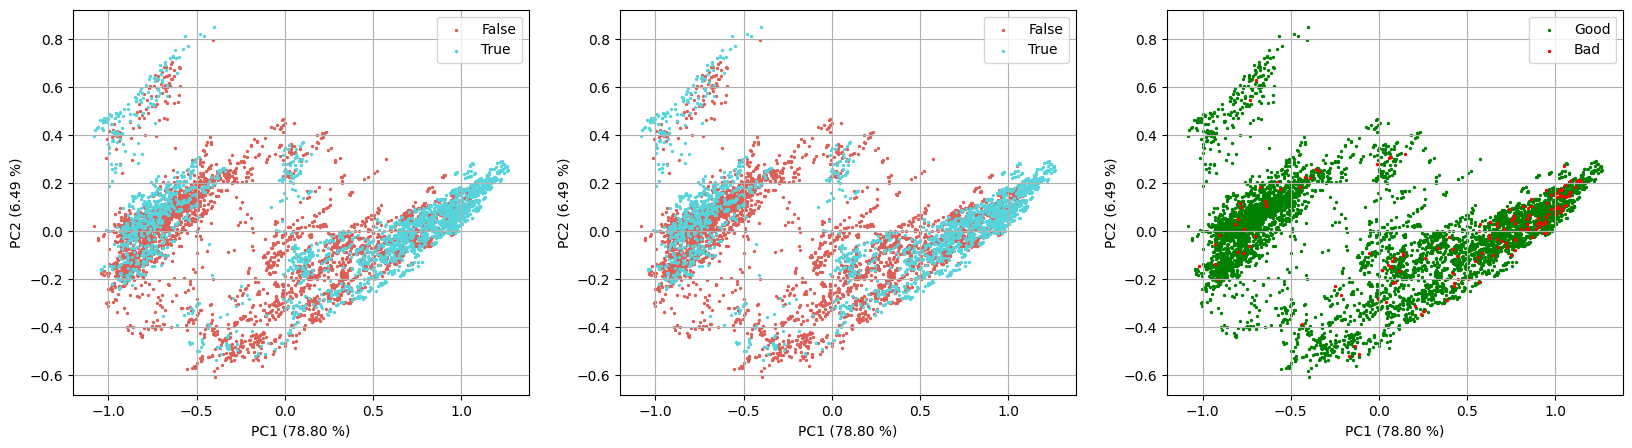
\includegraphics[width=\textwidth]{assets/design/pca-scatter-online-anomaly60-spectral.png}
        \caption{}
    \end{subfigure}
    \caption{PCA 2 components to visualize results and mistakes of online learning on all features}
\end{figure}


\section{Vibration measurement plan}

\subsection{Machinery}
% Enum list

\begin{figure}[ht]
    \centering
    \begin{subfigure}[b]{0.49\textwidth}
    		\centering
        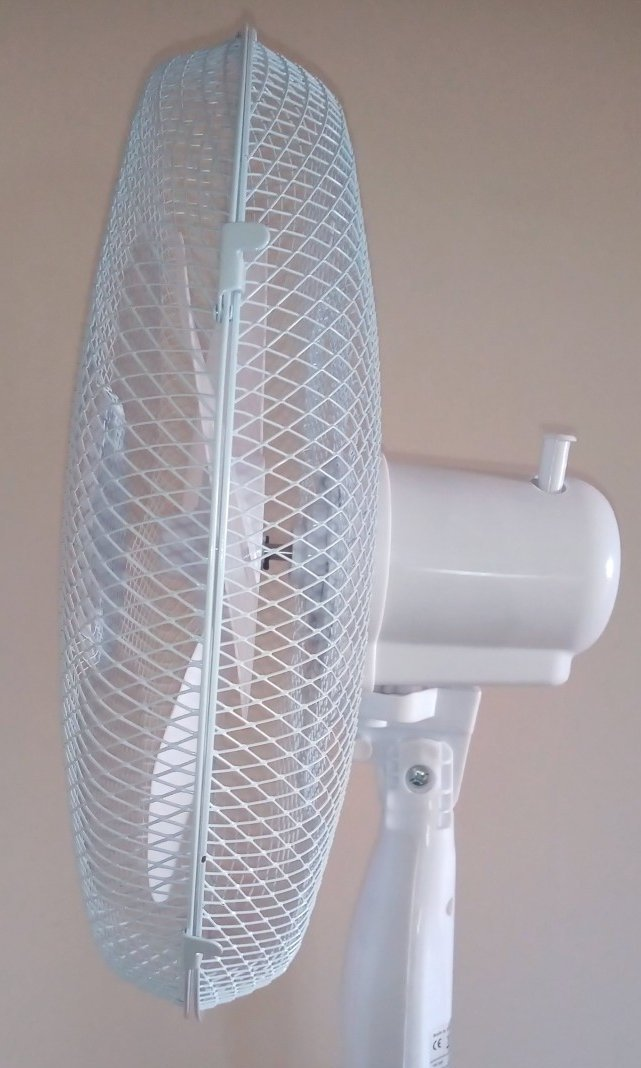
\includegraphics[width=0.5\textwidth]{assets/design/machine-fan.jpg}
        \caption{Stand fan Kalorik}
    \end{subfigure}
    \hfill
    \begin{subfigure}[b]{0.49\textwidth}
    		\centering
        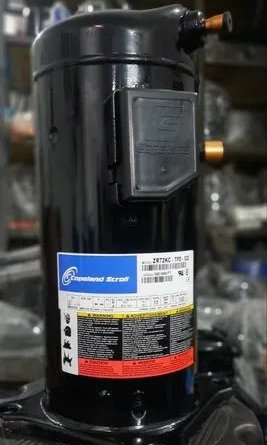
\includegraphics[width=0.5\textwidth]{assets/design/machine-compressor.jpg}
        \caption{Scroll compressor Copeland}
    \end{subfigure}
    \begin{subfigure}[b]{0.49\textwidth}
    		\centering
        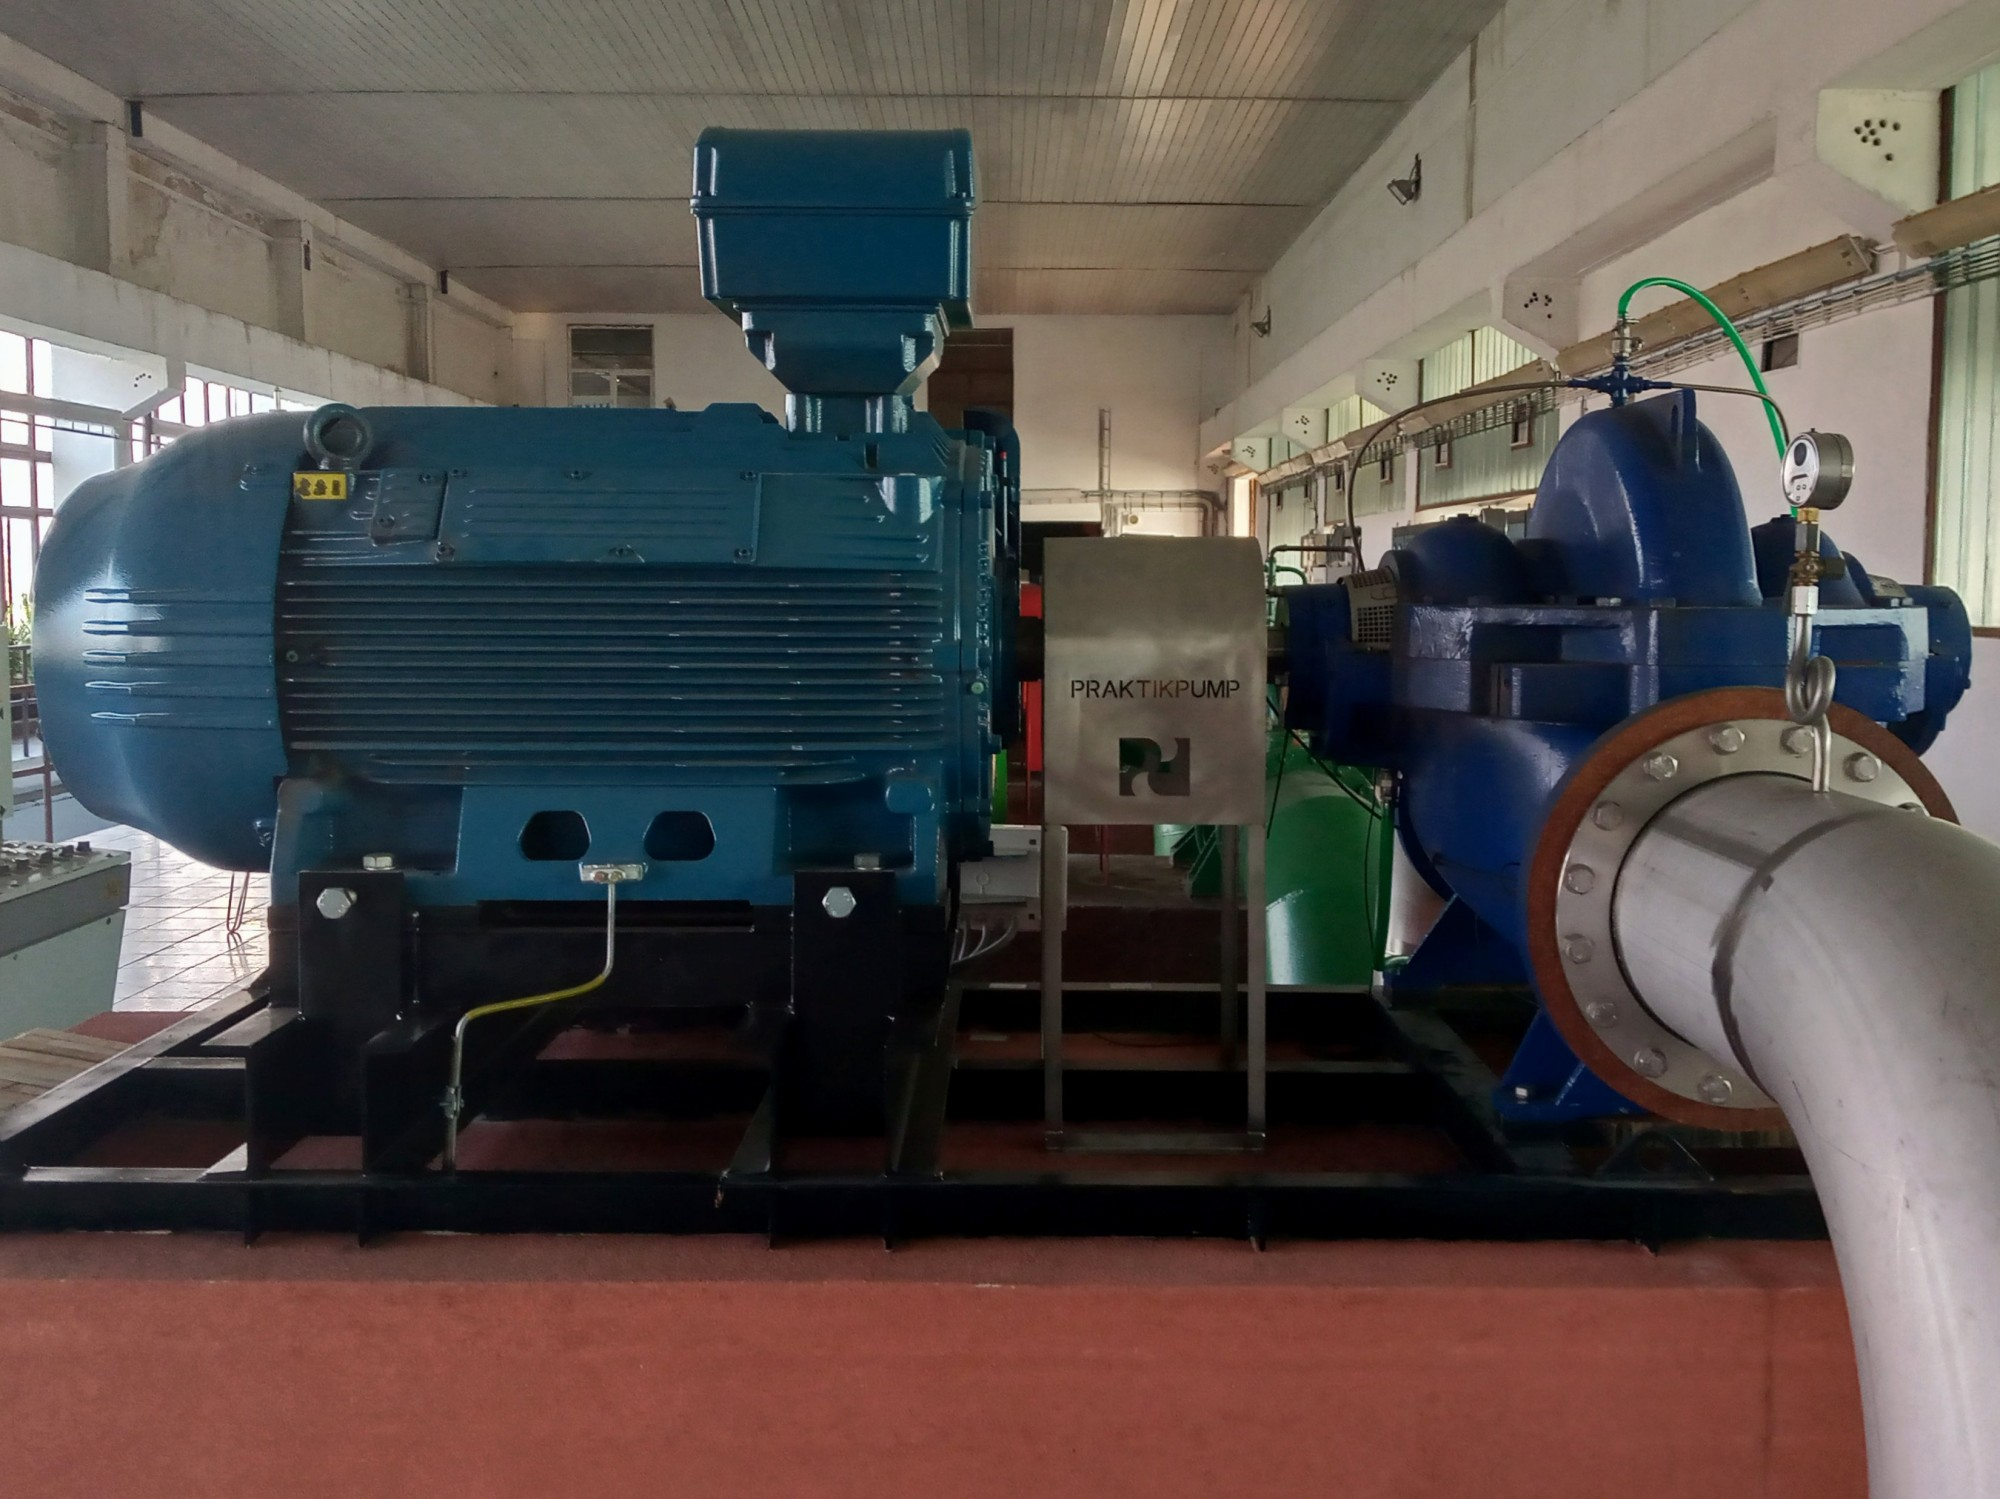
\includegraphics[width=\textwidth]{assets/design/machine-ksb-pump.jpg}
        \caption{Water pump KSB Omega}
    \end{subfigure}
    \hfill
    \begin{subfigure}[b]{0.49\textwidth}
    		\centering
        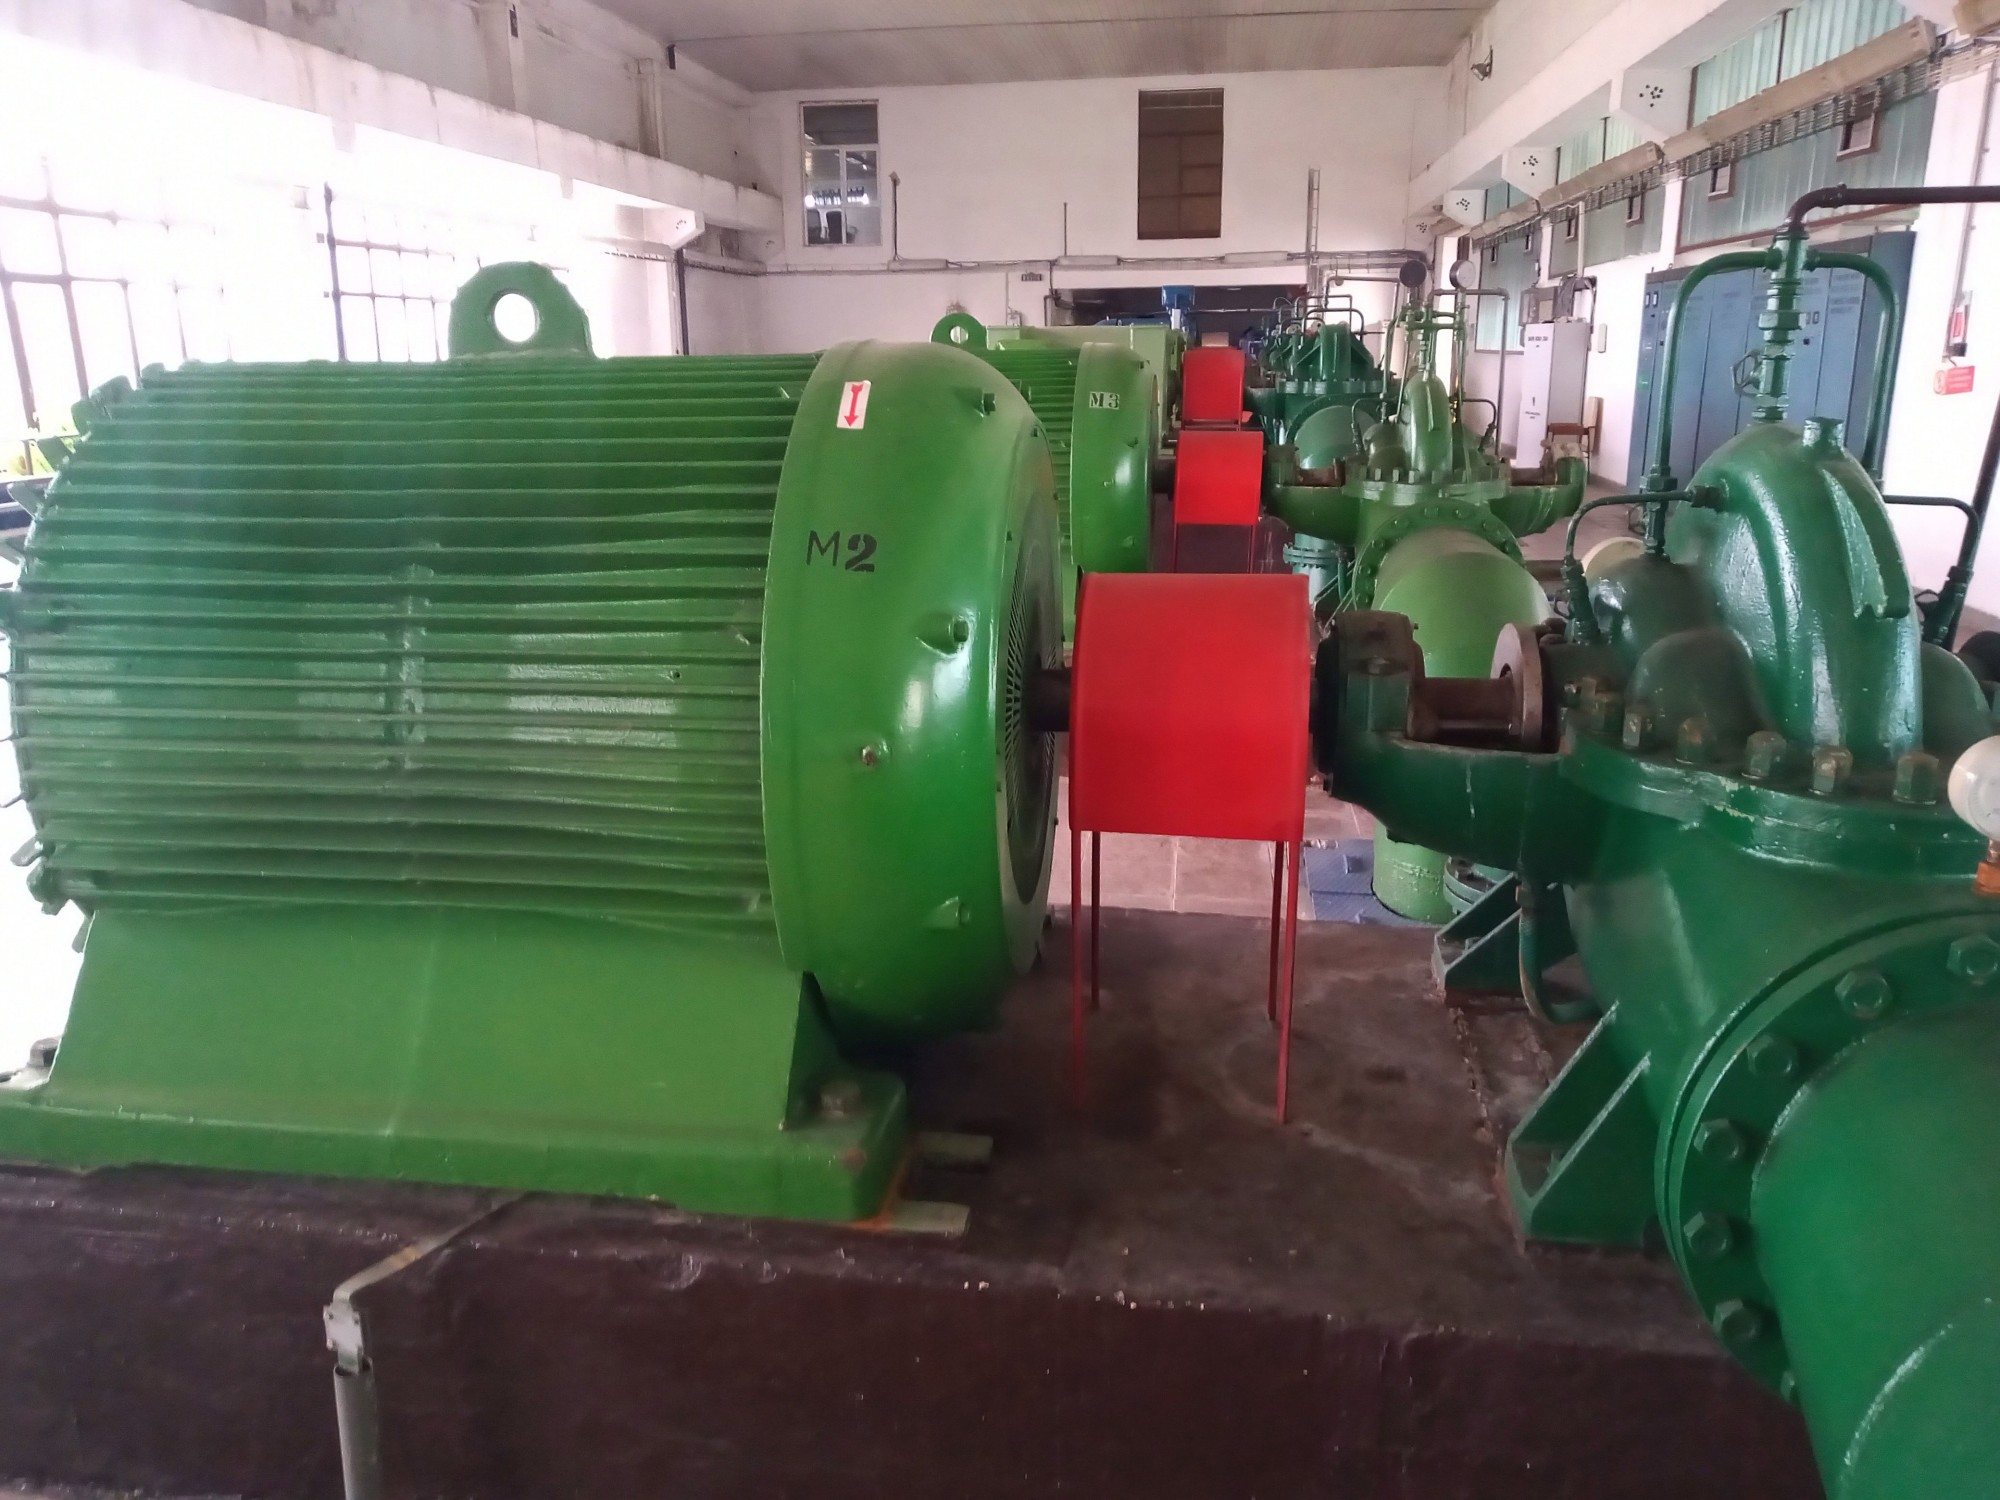
\includegraphics[width=\textwidth]{assets/design/machine-sigma-pump.jpg}
        \caption{Water pump Sigma}
    \end{subfigure}
    \caption{Machine}
\end{figure}


\subsection{Sensors}

\begin{table}[ht]
\renewcommand{\arraystretch}{1.2}
\begin{tabular}{|l|l|l|}
\hline
\textbf{Accelerometer}                           & \textbf{ADXL335} & \textbf{IIS3DWB}   \\ \hline
\textbf{Vendor}                                  & Analog Devices   & STMicroelectronics \\ \hline
\textbf{Bus}                                     & Analog           & SPI                \\ \hline
\textbf{Axis}                                    & 3                & 1 or 3             \\ \hline
\textbf{Range} (g)                               & $\pm$ 3          & $\pm$ 2 to 16      \\ \hline
\textbf{Bandwidth} (kHz)                         & 0.55             & 5 - 6.3            \\ \hline
\textbf{Sensitivity}                             & 300 mV/g         & 0.061 mg/LSB       \\ \hline
\textbf{Noise density} ($\mu g / \sqrt{\mathrm{Hz}}$ rms) & 150 - 300        & 75                 \\ \hline
\textbf{Microcontroller}                         & Beaglebone Black & ESP32-PoE-ISO      \\ \hline
\textbf{CPU SoC}                                 & TI Sitara AM3358 & ESP32-WROOM-32     \\ \hline
\textbf{Output data rate} (kHz)                  & 2.5              & 26.7               \\ \hline
\textbf{ADC resolution} (bit)                    & 12               & 16                 \\ \hline
\textbf{FIFO}                                    & -                & 3 kB (512 samples) \\ \hline
\end{tabular}
\caption{Accelerometers}
\end{table}


\begin{figure}[h]
	\centering
	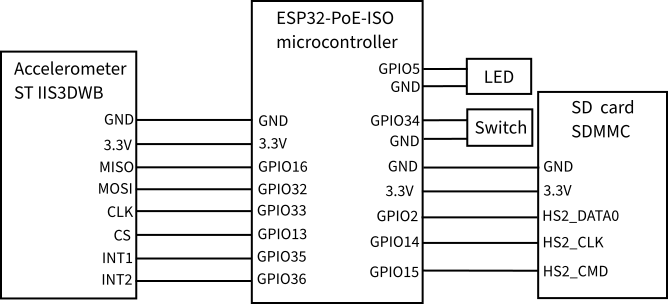
\includegraphics[width=\textwidth]{assets/design/hw-block-schematic.png}
	\caption{Sensor unit hardware block diagram}
\end{figure}

\subsection{Preliminary measurements}
\begin{figure}[ht]
    \centering
    \begin{subfigure}[b]{0.44\textwidth}
        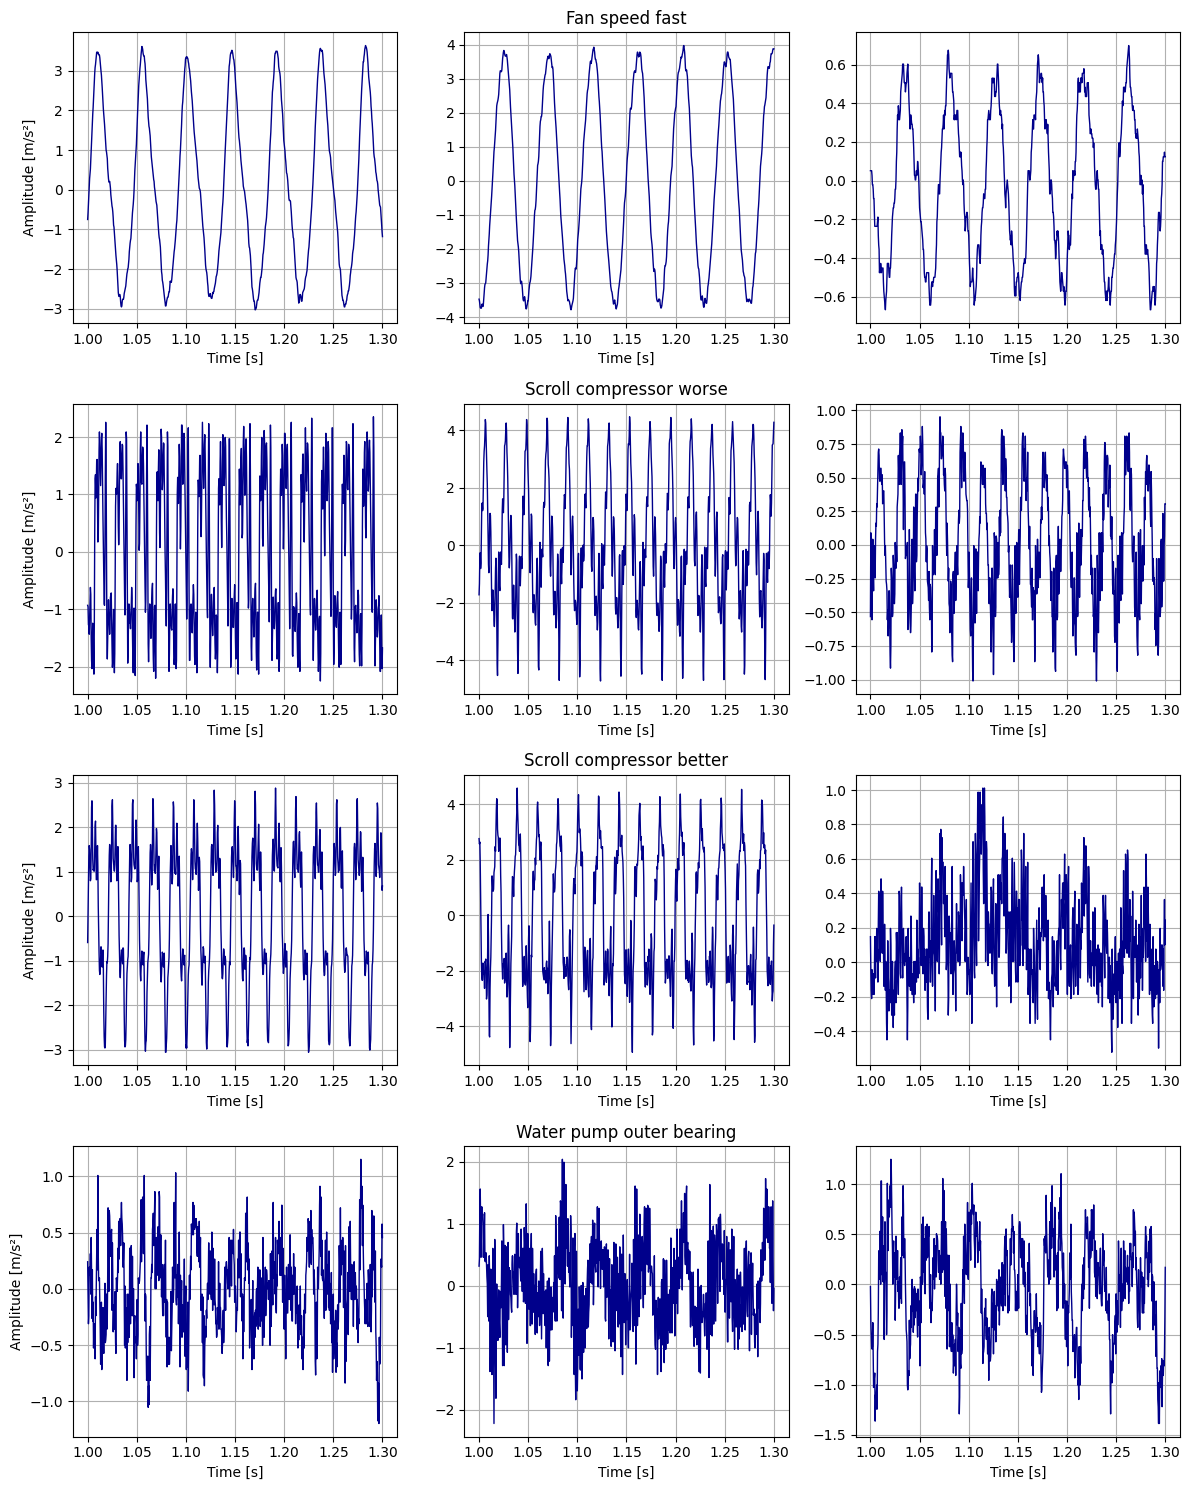
\includegraphics[width=\textwidth]{assets/design/EDA-custom-dataset-temporal.png}
        \caption{Temporal domain waveforms in all spatial directions with 300 ms duration}
    \end{subfigure}
    \hfill
    \begin{subfigure}[b]{0.55\textwidth}
        \includegraphics[width=\textwidth]{assets/design/EDA-custom-dataset-spectral-X-axis.png}
        \caption{Spectral domain in x accelerometer axis. FFT with Hann window of length $2^{10}$ ($\approx 409$ ms)}
    \end{subfigure} 
    \caption{Signals at 5 s timestamp}
\end{figure}






\newpage
\section{Machine learning pipeline}
\begin{enumerate}
    \itemsep0pt
    \item Detrending
    \item (Optional) Adaptive noise cancellation of the background interference
    \item Vector of all features
    \begin{itemize}
        \itemsep0pt
        \item Time domain: statistical measures (Tab.~\ref{tab:td-features})
        \item Frequency domain: PSD estimation with FFT and Welch averaging with the resolution of 1 Hz combined with Hann window (Tab.~\ref{tab:fd-features})
    \end{itemize}
    \item Feature selection on evaluation datasets and experimental measurements from the factory to prune away irrelevant features with pearson correlation, Fisher score, and mutal information.
    \item Model evaluation and comparison of novelty detection methods and precision of classification with different sets of predictors. The range of optimal parameters will be found for the DenStream ($\mu$, $\epsilon$, $beta$, $\lambda$), Half-Space Trees (window size, ensemble size), and kNN (distance metric, $k$ neighbours). Evaluation metrics associated with confusion matrices will be used like accuracy, precision, true positive rate, and false positive rate.
\end{enumerate}

\begin{figure}[h]
\centering
\includegraphics[width=0.9\textwidth]{assets/analysis/ml-lifecycle.png}
\caption{Machine learning lifecycle of feature discovery}
\end{figure}


\section{Infrastructure deployment}
Future work: engineer new feature, deploy, tweek models, validate on real dataset

 \begin{itemize}
 \itemsep0pt
\item \textbf{Input:} Samples from three-axis MEMS accelerometers, RPM tachometer, Noise background
\item \textbf{Output:} machine health status / type of fault
\item \textbf{Output on demand}: Control chart of trend features
\end{itemize}

\begin{enumerate}
\itemsep0pt
\item \textbf{Accelerometer} - MEMS accelerometers will be placed on at least two distinct measurement points in two perpendicular axes and one sensor in the machine base for denoising purposes. Rotational speed has to be captured at the same time too. The sampling frequency shall be around 2 kHz if unbalance and looseness is to be identified, and 10 kHz if bearing faults are also of interest. The range of overall rms vibrations is not expected to exceed 30 mm/s according to the vibration severity chart.
\item \textbf{Acquisition interval} - sensor units will be triggered in regular intervals (every 15 - 60 minutes) to collect vibration recordings from the band saw (or another machine of choice). The machine has to be under the same load conditions every time is recording is active. 
\item \textbf{Features} - most relevant features are computed and compared to recent measurements. If there is a statistically significant change the whole summary is sent, otherwise keep-alive notification is sent. 
\item \textbf{Wireless network} - earlier design decision has been made to establish wireless connections. Therefore, the sensor unit will send data over Wifi (IEEE 802.11), or Thread with IEEE 802.15.4 over 2.4 GHz or 868 MHz frequency bands. The application protocol shall be Constrained Application Protocol (CoAP). The messages will be encoded by Concise Binary Object Representation (CBOR) or MessagePack which provides the best compression ratio and is widely supported.
\item \textbf{Time series database} - stores history of trend values. Raw vibration measurements can be requested by the operator at any time but are available and delayed according to transfer speeds and other network constraints. The promissing database technologies is TimescaleDB.
\item \textbf{Diagnosis panel} - continuously updates the anomaly detection and classification models with the introduction of annotations to notify the operator about observed faults and imminent failure of the machine. The dashboard is provided to display the current status of multiple machines.
\end{enumerate}

\begin{figure}[h]
\centering
\includegraphics[width=0.7\textwidth]{assets/design/sensor-network.png}
\caption{Sensor network components}
\end{figure}
